\documentclass[11pt,a4paper]{article}

% Packages
\usepackage[utf8]{inputenc}
\usepackage[spanish, es-tabla]{babel}
\usepackage{parskip}
\usepackage{enumerate}
\usepackage{graphicx}
\usepackage{subfigure}
\usepackage{float}
\usepackage{amsmath}


\usepackage[bookmarks=true,
					 bookmarksnumbered=false,
					 bookmarksopen=false,
					 colorlinks=true,
					 allcolors=blue,
					 urlcolor=blue]{hyperref}

\usepackage[ruled]{algorithm2e}
\SetKwInOut{Parameter}{parameter}

\usepackage{array}
\newcolumntype{N}{>{\centering\arraybackslash}m{0.5cm}}
\newcolumntype{M}{>{\centering\arraybackslash}m{1cm}}

\usepackage[left=2cm, right=2cm, top=2cm, bottom=2cm]{geometry}

\begin{document}\pagenumbering{arabic}
\begin{titlepage}
\centering
\includegraphics[width=0.15\textwidth]{/Users/pedrors/Desktop/DGIIM/Latex/UGR}\par\vspace{1cm}
{\scshape\LARGE Universidad de Granada \par}
\vspace{1cm}
{\Huge\bfseries Práctica 2.b\par}
{\Large\bfseries Técnicas de Búsquedad basadas en Poblaciones para el Problema del aprendizaje de Pesos en Características\par}
\vspace{1.5cm}
{\huge\bfseries Metaheurísticas\par}
{\large\bfseries Grupo 2 (Lunes)\par}
\vspace{2cm}
{\Large\itshape Pedro Ramos Suárez\par}
{\large\itshape 76591270M\par}
{\large\itshape pedrors@correo.ugr.es\par}
\vfill
Doble Grado de Ingeniería Informática y Matemáticas
\vfill
{\large \today \par}
\author{A}
\end{titlepage}

\tableofcontents
\newpage
\section{Problema de Aprendizaje de Pesos en Características}

\subsection{Descripción del problema}

El problema consiste en optimizar el rendimiento de un clasificador basado en el vecino más cercano a partir de la inclusión de pesos asociados a las características del problema.

El clasificador utilizado es el 1-NN (1 vecino más cercano), el cuál consiste en asignar a cada nuevo la misma etiqueta que a su vecino más cercano. Para ello, utilizamos la distancia euclídea modificada por unos pesos asociados a cada característica:
$$d(e_{1}, e_{2}) = (\sum_{i=1}^{n} w_{i} \cdot (e_{1}^{i} - e_{2}^{i})^{2})^{\frac{1}{2}}$$
donde $n$ es el número de características de los datos, y $W = (w_{1}, \dots, w_{n})$ el vector de números reales entre 0 y 1 que define el peso que pondera cada una de las características.

La variante que intentaremos optimizar será la agregación, que combina tanto la precisión como la complejidad del clasificador, definida como:
\begin{equation} \label{eq:objetivo}
\text{Agregación}(W) = \alpha \cdot \text{Tasa\_clas}(W) + (1 - \alpha) \cdot \text{Tasa\_red}(W)
\end{equation}
donde:
\begin{equation} \label{eq:clas}
\text{Tasa\_clas} = 100 \cdot \frac{\text{nº de instancias bien clasificadas en T}}{\text{nº de instancias en T}}
\end{equation}
\begin{equation} \label{eq:red}
\text{Tasa\_red} = 100 \cdot \frac{\text{nº de valores } w_{i} < 0.1}{\text{nº de características}}
\end{equation}

siendo $T$ el conjunto de datos sobre los que se evalúa el clasificador, y $\alpha$ es un número real entre 0 y 1 que pondera la importancia entre acierto y la reducción de la solución.

\subsection{Datos utilizados}

Los datos utilizados serán:
\begin{enumerate}
\item \textbf{Ionosphere}: Conjunto de datos de radar, formado por 351 ejemplos con 34 características clasificados en dos clases.
\item \textbf{Parkinsons}: Conjunto de datos orientados a distinguir entre la presencia y ausencia de la enfermedad de Parkinson en una serie de pacientes, formado por 195 ejemplos con 22 características clasificados en dos clases.
\item \textbf{Spectf-heart}: Conjunto de datos de detección de enfermedades cardíacas a partir de imágenes médicas de termografía computerizada del corazón, formada por 349 ejemplos con 44 características clasificados en dos clases.
\end{enumerate}

\newpage
\section{Aplicación de los algoritmos} \label{sec:algorithms}
Todos los algoritmos utilizados para resolver este problema tienen como entrada la matriz de datos de las características $D = (k \times n)$, y el vector de etiquetas asociadas a dicha matriz $y = (y_{1}, \dots, y_{k})$, donde $k$ es el número de ejemplos, y $n$ el número de características. Dependiendo del algoritmo, estos datos pueden ser todos los leídos, o sólo un subconjunto de entrenamiento.

Para representar las soluciones, utilizaremos un vector de números reales entre 0 y 1, $W = (w_{1}, \dots, w_{n})$, que define el peso que pondera cada una de las características.

La evaluación de la calidad de una solución se hará como indicada en \eqref{eq:objetivo}, tomando como $\alpha = 0.5$, es decir, dándole la misma importancia al acierto y a la reducción de las características, por lo que será de la forma:
$$\text{Agregación}(W) = 0.5 \cdot \text{Tasa\_clas}(W) + 0.5 \cdot \text{Tasa\_red}(W) = \frac{\text{Tasa\_clas}(W) + \text{Tasa\_red}(W)}{2}$$

\subsection{Algoritmos para evaluar las soluciones}

El pseudocódigo de la función para calcular la tasa de clasificación es: \\
\begin{algorithm}[H]
	\caption{{\sc Tasa\_Clas} calcula la tasa de clasificación de una solución.}
	\KwIn{El conjunto de etiquetas reales $Y$.}
	\KwIn{El conjunto de etiquetas obtenidas de la predicción del vecino más cercano $P$.}
	\KwOut{La tasa de clasificación como se describe en \eqref{eq:clas}.}
	
	$clas \gets 0$ \;
	\For{$i=0$ \textbf{to} $length(Y)$} {
		\If{$Y[i] = P[i]$} {
			$clas \gets clas + 1$ \;
		}
	}
	$output \gets clas / length(Y)$ \;
	\Return{$output$} \;
\end{algorithm}

El pseudocódigo de la función para calcular la tasa de reducción es: \\
\begin{algorithm}[H]
	\caption{{\sc Tasa\_Red} calcula la tasa de reducción de una solución.}
	\KwIn{El conjunto de pesos $W$.}
	\KwIn{El conjunto de etiquetas obtenidas de la predicción del vecino más cercano $P$.}
	\KwOut{La tasa de clasificación como se describe en \eqref{eq:red}.}
	
	$red \gets 0$ \;
	\For{$w$ \textbf{in} $W$} {
		\If{$w < 0.1$} {
			$red \gets red + 1$ \;
		}
	}
	$output \gets red / length(W)$ \;
	\Return{$output$} \;
\end{algorithm}

Por último, el pseudocódigo de la función de agregación obtenido a partir de la tasa de clasificación y la tasa de reducción es: \\
\begin{algorithm}[H] \label{alg:agregation}
	\caption{{\sc Agregacion} calcula la agregación de una solución.}
	\KwIn{El conjunto de pesos $W$.}
	\KwOut{La agregación como se describe en \eqref{eq:objetivo}.}
	
	$clas \gets \operatorname{tasa\_clas}(W)$ \;
	$red \gets \operatorname{tasa\_red}(W)$ \;
	$output \gets (clas + red)/2$ \;
	\Return{$output$} \;
\end{algorithm}

\subsection{Algoritmos para calcular las distancias}

Utilizaremos la distancia euclídea o una variante que modifica la importancia de cada componente según los pesos.

El pseudocódigo para la distancia euclídea es: \\
\begin{algorithm}[H]
	\caption{{\sc Eulcidean} calcula la distancia entre dos puntos.}
	\KwIn{Un vector con las coordenadas del primer punto $P$.}
	\KwIn{Un vector con las coordenadas del segundo punto $Q$.}
	\KwOut{La distancia entre los dos puntos.}
	
	$dist \gets 0$ \;
	\For{$i=0$ \textbf{to} $length(P)$} {
		$dist \gets dist + (P[i] - Q[i])^{2}$ \;
	}
	$output \gets sqrt(dist)$ \;
	\Return{$output$} \;
\end{algorithm}

El pseudocódigo para la distancia euclídea modificada por el vector de pesos es: \\
\begin{algorithm}[H]
	\caption{{\sc Weighted\_Eulcidean} calcula la distancia entre dos puntos.}
	\KwIn{Un vector de pesos $W$.}
	\KwIn{Un vector con las coordenadas del primer punto $P$.}
	\KwIn{Un vector con las coordenadas del segundo punto $Q$.}
	\KwOut{La distancia entre los dos puntos.}
	
	$dist \gets 0$ \;
	\For{$i=0$ \textbf{to} $length(W)$} {
		\If{$W[i] > 0.1$} {
			$dist \gets dist + W[i] (P[i] - Q[i])^{2}$ \;
		}
	}
	$output \gets sqrt(dist)$ \;
	\Return{$output$} \;
\end{algorithm}

\subsection{Algoritmos para predecir las etiquetas}

Tenemos dos casos:
\begin{enumerate}
\item El conjunto de datos está dividido en entrenamiento y test. Entonces predeciremos las etiquetas del conjunto de test a partir de los resultados obtenidos en entrenamiento.
\item Los datos no están divididos en entrenamiento y test. Entonces aplicaremos el algoritmo \emph{leave-one-out}, que predice una etiqueta a partir de todos los demás datos.
\end{enumerate}

Para el pseudocódigo utilizaremos la versión de la distancia euclídea con pesos. Sin embargo, el caso que no los utiliza sería casi idéntico, pero sin tomar el vector de pesos como entrada, y utilizando la función \emph{euclidean} en lugar de \emph{weighted\_euclidean}.

El pseudocódigo para el primer caso, en el que tenemos los datos separados en entrenamiento y test, es: \\
\begin{algorithm}[H] \label{alg:predictlabel}
	\caption{{\sc Predict\_Label} predice las etiquetas.}
	\KwIn{Una matriz de datos de test $X\_test$.}
	\KwIn{Una matriz de datos de entrenamiento $X$.}
	\KwIn{Un vector con las etiquetas de entrenamiento $Y$.}
	\KwIn{El vector de pesos $W$.}
	\KwOut{Un vector con la predicción de etiquetas de los datos de test.}
	
	$Y\_pred \gets \{\}$ \;
	\For{$x$ \textbf{in} $X\_test$} {
		$min\_dist \gets length(x)$ \;
		$neighbour \gets 0$ \;
		\For{$i=0$ \textbf{to} $length(X)$} {
			$dist \gets \operatorname{weighted\_euclidean}(x, X[i], W)$ \;
			\If{$dist < min\_dist$} {
				$min\_dist \gets dist$ \;
				$neightbour \gets i$ \;
			}
		}
		$Y\_pred \gets Y\_pred \cup \{neighbour\}$ \;
	}
	\Return{$Y\_pred$} \;
\end{algorithm}

Nótese que inicializamos la distancia mínima como el la longitud de $x$, es decir, el número de características. Esto se debe a que como los datos están normalizados, la distancia siempre será menor.

El pseudocódigo para el segundo caso, \emph{leave-one-out}, en el que tenemos un único conjunto de datos, es:
\begin{algorithm}[H] \label{alg:leaveoneout}
	\caption{{\sc Leave\_One\_Out} predice las etiquetas.}
	\KwIn{Una matriz de datos $X$.}
	\KwIn{Un vector con las etiquetas $Y$.}
	\KwIn{El vector de pesos $W$.}
	\KwOut{Un vector con la predicción de etiquetas.}
	
	$Y\_pred \gets \{\}$ \;
	\For{$x$ \textbf{in} $X$} {
		$min\_dist \gets length(x)$ \;
		$neighbour \gets 0$ \;
		\For{$i=0$ \textbf{to} $length(X)$} {
			\If{$x \neq X[i]$} {
				$dist \gets \operatorname{weighted\_euclidean}(x, X[i], W)$ \;
				\If{$dist < min\_dist$} {
					$min\_dist \gets dist$ \;
					$neightbour \gets i$ \;
				}
			}
		}
		$Y\_pred \gets Y\_pred \cup \{neighbour\}$ \;
	}
	\Return{$Y\_pred$} \;
\end{algorithm}

\subsection{Otros algoritmos}

Por último, sólo nos queda un algoritmo que merece la pena mencionar, que es el que separa los datos en entrenamiento: \\
\begin{algorithm}[H]
	\caption{{\sc Train\_Test\_Split} divide los datos en entrenamiento y test.}
	\KwIn{Una matriz de datos $X$.}
	\KwIn{Un vector con las etiquetas $Y$.}
	\KwIn{Un entero que indica el número de conjuntos en el que dividir los datos $n$.}
	\KwIn{Un entero que indica qué conjunto es de test y cuáles de entrenamiento $k$.}
	\KwOut{Un vector con los datos de entrenamiento.}
	\KwOut{Un vector con los datos de test.}
	\KwOut{Un vector con las etiquetas de entrenamiento.}
	\KwOut{Un vector con las etiquetas de test.}
	
	$X\_train \gets \{\}$ \;
	$X\_test \gets \{\}$ \;
	$Y\_train \gets \{\}$ \;
	$Y\_test \gets \{\}$ \;
	$size \gets length(X) / n$ \;
	$remain \gets length(X) \% n$ \;
	\uIf{$k < remain$} {
		$begin \gets (size + 1)$ \;
		$end \gets begin + (size + 1)$ \;
	} \uElseIf{$k == remain$} {
		$begin \gets (size + 1)$ \;
		$end \gets begin + size$ \;
	} \Else {
		$begin \gets size$ \;
		$end \gets begin + size$ \;
	}
	\For{$i=0$ \textbf{to} $length(X)$} {
		\uIf{$i < begin$ \textbf{or} $i > begin$} {
			$X\_train \gets X\_train \cup X[i]$ \;
			$Y\_train \gets Y\_train \cup Y[i]$ \;
		} \Else{
			$X\_test \gets X\_test \cup X[i]$ \;
			$Y\_test \gets Y\_test \cup Y[i]$ \;
		}
	}
	\Return{$X\_train$} \;
	\Return{$X\_test$} \;
	\Return{$Y\_train$} \;
	\Return{$Y\_test$} \;
\end{algorithm}

En caso de que el número de datos sea múltiplo del número de particiones, todas estas tendrán el mismo tamaño. En caso de que no lo sea, los primeros conjuntos de test tendrán un elemento extra.

\subsection{Algoritmos utilizados en los algoritmos genéticos}\label{sec:gen_alg}

La representación de las soluciones empleadas están explicadas en la sección \ref{sec:algorithms}.

La función objetivo es la agregación, definida en el algoritmo \ref{alg:agregation}.

En los algoritmos genéticos utilizamos un algoritmo para inicializar los cromosomas a soluciones aleatorias con una distribución uniforme entre 0 y 1: \\
\begin{algorithm}[H]
	\caption{{\sc Initialize} inicializa una solución.}
	\KwIn{Un entero con el número de cromosomas a inicializar $size$.}
	\KwIn{Un generador de números aleatorios con distribución uniforme entre 0 y 1, $generator$.}
	\KwOut{Una matriz con los cromosomas inicializados.}
	
	$w \gets \{\}$ \;
	\For{$i$ \textbf{in} $\{0, \dots, size\}$}{
		$w \gets w \cup \operatorname{generator}()$ \;
	}	
	
	\Return{$w$} \;
\end{algorithm}

Para seleccionar los padres que cruzaremos, utilizamos un mismo algoritmo para el caso estacionario y el caso generacional, basado en el torneo binario, con la diferencia de que el caso generacional creamos tantos padres como cromosomas, y en el caso estacionario sólo generamos dos. Dicho algoritmo es: \\
\begin{algorithm}[H]
	\caption{{\sc Selection} selecciona los cromosomas a cruzar.}
	\KwIn{Una matriz con los cromosomas $solutions$.}
	\KwIn{Un vector con el ``fitness'' de los cromosomas $fitness$.}
	\KwIn{Un entero con el número de cromosomas a obtener $size$.}
	\KwOut{Una matriz con los cromosomas a cruzar.}
	
	$parents \gets \{\}$ \;
	\For{$i$ \textbf{in} $\{0, \dots, size\}$}{
		$random1 \gets \operatorname{rand}() \% length(solutions)$ \;
		$random2 \gets \operatorname{rand}() \% length(solutions)$ \;
		
		
		\uIf{$fitness[random1] > fitness[random2]$}{
			$parents \gets parents \cup solutions[random1]$ \;
		}\Else{
			$parents \gets parents \cup solutions[random2]$ \;
		}
	}	
	
	\Return{$parents$} \;
\end{algorithm}

Para el cruce, tenemos dos casos. El primero de ellos es utilizando Blx-$\alpha$, con $\alpha = 0.3$, con una probabilidad de cruce de $0.7$. Este algoritmo es: \\
\begin{algorithm}[H]
	\caption{{\sc CrossBlx} cruza los cromosomas utilizando Blx.}
	\KwIn{Una matriz con los cromosomas $solutions$.}
	\KwIn{Un generador de números aleatorios con distribución uniforme entre 0 y 1, $generator$.}
	\KwOut{Una matriz con los cromosomas tras el cruce.}
	
	$newSolutions \gets \{\}$ \;
	$crosses \gets 0.7 \cdot length(solutions) \slash 2$ \;
	\For{$i$ \textbf{in} $\{0, \dots, crosses\}$}{
		$parent1 \gets 2 \cdot i$ \;
		$parent2 \gets (2 \cdot i + 1) \% length(solutions)$ \;
		
		\For{$j$ \textbf{in} $\{0, 1\}$}{
			$w \gets \{\}$ \;
			\For{$k$ \textbf{in} $length(solutions[parent1])$}{
				\uIf{$solutions[parent1][k] < solutions[parent2][k]$}{
					$min \gets solutions[parent1][k]$ \;
					$max \gets solutions[parent2][k]$ \;
				}\Else{
					$min \gets solutions[parent2][k]$ \;
					$max \gets solutions[parent1][k]$ \;
				}
				$min \gets min + 0.3 \cdot (max - min)$ \;
				$max \gets max + 0.3 \cdot (max - min)$ \;
				$gene \gets min + \operatorname{generator}() \cdot (max - min)$ \;
				\uIf{$gene < 0$}{
					$gene \gets 0$ \;
				}\ElseIf{$gene > 1$}{
					$gene \gets 1$ \;
				}
				$w \gets w \cup gene$ \;
			}
			$newSolutions \gets newSolutions \cup w$ \;
		}
	}
	
	\For{$i$ \textbf{in} $\{2 \cdot crosses, \dots, length(solutions)\}$}{
		$newSolutions \gets newSolutions \cup solutions[i]$ \;
	}
	
	\Return{$newSolutions$} \;
\end{algorithm}

Para el cruce aritmético, el algoritmo es similar, pero los genes de los hijos son la media de los genes de los padres. Sin embargo, como dos padres generan dos hijos, y estos dos hijos se generaría de igual forma, obtendríamos los hijos idénticos, por lo que modificamos este algoritmo para que, en lugar de ser la media entre ambos padres, sea un valor aleatorios entre ambos padres, pero no necesariamente la media. El algoritmo es: \\
\begin{algorithm}[H]
	\caption{{\sc CrossCa} cruza los cromosomas utilizando cruce aritmético.}
	\KwIn{Una matriz con los cromosomas $solutions$.}
	\KwIn{Un generador de números aleatorios con distribución uniforme entre 0 y 1, $generator$.}
	\KwOut{Una matriz con los cromosomas tras el cruce.}
	
	$newSolutions \gets \{\}$ \;
	$crosses \gets 0.7 \cdot length(solutions) \slash 2$ \;
	\For{$i$ \textbf{in} $\{0, \dots, crosses\}$}{
		$parent1 \gets 2 \cdot i$ \;
		$parent2 \gets (2 \cdot i + 1) \% length(solutions)$ \;
		$alpha \gets \operatorname{generator}()$ \;
		
		\For{$j$ \textbf{in} $\{0, 1\}$}{
			$w \gets \{\}$ \;
			\If{$j == 1$}{
				$\alpha \gets 1 - \alpha$ \;
			}
			\For{$k$ \textbf{in} $length(solutions[parent1])$}{
				$gene \gets alpha \times solutions[parent1][k] + (1 - \alpha) solutions[parent2][k]$ \;
				$w \gets w \cup gene$ \;
			}
			$newSolutions \gets newSolutions \cup w$ \;
		}
	}
	
	\For{$i$ \textbf{in} $\{2 \cdot crosses, \dots, length(solutions)\}$}{
		$newSolutions \gets newSolutions \cup solutions[i]$ \;
	}
	
	\Return{$newSolutions$} \;
\end{algorithm}

Por último, nos queda ver la mutación, que ocurre con una probabilidad de $0.1$. El algoritmo utiliza la función $permutation$, que únicamente toma como parámetro un entero $n$, y devuelve un array con valores entre $\{0, \dots, n\}$ pero con orden aleatorio. Debido a la simplicidad de este algoritmo, no entraré en detalle en su funcionamiento. El algoritmo de mutación es: \\
\begin{algorithm}[H]
	\caption{{\sc Mutation} muta los genes.}
	\KwIn{Una matriz con los cromosomas $solutions$.}
	\KwIn{Un generador de números aleatorios con distribución normal de media 0 y varianza $0.3^{2}$, $generator$.}
	\KwOut{Una matriz con los cromosomas mutados.}
	
	$mutations \gets 0.1 \cdot length(solutions) \cdot length(solutions[0])$ \;
	$perm \gets \operatorname{permutation}(length(solutions) \cdot length(solutions[0]))$ \;
	\For{$i$ \textbf{in} $\{0, \dots, mutations\}$}{
		$chromosome \gets perm[i] \slash length(solutions[0])$ \;
		$gene \gets perm[i] \% length(solutions[0])$ \;
		
		$solutions[chromosome][gene] \gets solutions[chromosome][gene] + \operatorname{generator}()$ \;
		
		\uIf{$solutions[chromosome][gene] < 0$}{
			$solutions[chromosome][gene] \gets 0$ \;
		}\ElseIf{$solutions[chromosome][gene] > 1$}{
			$solutions[chromosome][gene] \gets 1$ \;
		}
	}
	
	\Return{$solutions$} \;
\end{algorithm}

\newpage
\section{Descripción de los algoritmos}

\subsection{Algoritmos genéticos}

Para los cuatro algoritmos genéticos, la idea general es la misma: \\
\begin{algorithm}[H]
	\caption{{\sc Genetic\_Algorithm} algoritmo genético.}
	\KwIn{Una matriz con los caracteríssticas $x$.}
	\KwIn{Un vector con las etiquetas $y$.}
	\KwIn{El número de cromosomas $chromosomes$.}
	\KwIn{El número de iteraciones $iterations$.}
	\KwIn{El valor por debajo del cuál el peso se considera cero, $reduction$.}
	\KwIn{La probabilidad de mutación, $mutationChance$.}
	\KwOut{Una vector con los pesos de la solución.}
	
	$eval \gets 0$ \;
	$solutions \gets \operatorname{initialize}(chromosomes, length(w[0]))$ \;
	$fitness \gets \{\}$ \;
	$uniform \gets$ Un generador de distribución uniforme entre 0 y 1. \;
	$normal \gets$ Un generador de distribución normal de media 0 y varianza $0.3^{2}$. \;
	$newSolutions \gets \{\}$ \;
	
	\For{$i$ \textbf{in} $\{0, \dots, length(solutions)\}$}{
		$fitness \gets fitness \cup \operatorname{agregation}(solutions[i])$ \;
		$eval \gets eval + 1$ \;
	}
	
	\While{$eval < iterations$}{
		$size \gets 2$ \tcp{En el caso estacionario}
		$size \gets length(solutions)$ \tcp{En el caso generacional}
		$newSolutions \gets \operatorname{selection}(solutions, fitness, size)$ \;
		
		$newSolutions \gets \operatorname{cross}(newSolutions, uniform)$ \;
		$newSolutions \gets \operatorname{mutation}(newSolutions, normal)$ \;
		$solutions \gets \operatorname{replace}(solutions, newSolutions, fitness, eval)$ \;
		}
	
	$ind \gets 0$ \;
	$bestFitness \gets fitness[0]$ \;
	\For{$i$ \textbf{in} $\{1, \dots, length(fitness)\}$}{
		\If{$fitness[i] > bestFitness$}{
			$ind \gets i$ \;
			$bestFitness \gets fitness[i]$ \;
		}
	}
	
	\Return{$solutions[ind]$} \;
\end{algorithm}

El cruce utilizado puede ser el cruce aritmético o Blx, y todas las funciones utilizadas están definidas en \ref{sec:gen_alg}, con la excepción de $\operatorname{replace}$. Esta función depende de si estamos en el caso generacional o estacionario, siendo en el caso generacional: \\
\begin{algorithm}[H]
	\caption{{\sc Replace} algoritmo generacional elitista utilizado para reemplazar las soluciones.}
	\KwIn{Una matriz con los cromosomas de la generación previa $solutions$.}
	\KwIn{Una matriz con los cromosomas obtenidos del cruce y mutación $w$.}
	\KwIn{Un vector con la agregación de las soluciones $fitness$.}
	\KwIn{Número de evaluaciones realizadas $eval$.}
	\KwOut{Una matriz con los cromosomas para la siguiente generación.}
	
	$bestSolution \gets w[0]$ \;
	$bestFitness \gets fitness[0]$ \;
	\For{$i$ \textbf{in} $\{1, \dots, length(fitness)\}$}{
		\If{$fitness[i] > bestFitness$}{
			$bestSolution \gets w[i]$ \;
			$bestFitness \gets fitness[i]$ \;
		}
	}
	
	$solutions \gets w$ \;
	\For{$i$ \textbf{in} $\{0, \dots, length(solutions)\}$}{
		$fitness \gets fitness \cup \operatorname{agregation}(solutions[i])$ \;
		$eval \gets eval + 1$ \;
	}
	
	$ind \gets 0$ \;
	$worstFitness \gets fitness[0]$ \;
	\For{$i$ \textbf{in} $\{1, \dots, length(fitness)\}$}{
		\If{$fitness[i] < worstFitness$}{
			$ind \gets i$ \;
			$worstFitness \gets fitness[i]$ \;
		}
	}
	
	$solutions \gets solutions \setminus solutions[ind]$ \;
	$solutions \gets solutions \cup bestSolution$ \;
	
	\Return{$solutions$} \;
\end{algorithm}

En el caso estacionario, como sólo sustituimos dos soluciones, es algo más complejo: \\
\begin{algorithm}[H]
	\caption{{\sc Replace} algoritmo estacionario utilizado para reemplazar las soluciones.}
	\KwIn{Una matriz con los cromosomas de la generación previa $solutions$.}
	\KwIn{Una matriz con los dos cromosomas obtenidos del cruce y mutación $w$.}
	\KwIn{Un vector con la agregación de las soluciones $fitness$.}
	\KwIn{Número de evaluaciones realizadas $eval$.}
	\KwOut{Una matriz con los cromosomas para la siguiente generación.}
	
	$agregation1 \gets \operatorname{agregation}(w[0])$ \;
	$agregation2 \gets \operatorname{agregation}(w[1])$ \;
	$eval \gets eval + 2$ \;
	
	$minPos1 \gets 0$ \;
	$minPos2 \gets 1$ \;
	\If{$fitness[minPos2] < fitness[minPos1]$}{
		$minPos1 \gets 1$ \;
		$minPos2 \gets 0$ \;
	}
	\For{$i$ \textbf{in} $\{2, \dots, length(fitness)\}$}{
		\uIf{$fitness[i] < fitness[minPos1]$}{
			$minPos2 \gets minPos1$ \;
			$minPos1 \gets i$ \;
		} \ElseIf{$fitness[i] < fitness[minPos2]$}{
			$minPos2 \gets i$ \;
		}
	}
	
	\uIf{$agregation1 > agregation2$}{
		\uIf{$agregation1 > fitness[minPos2]$}{
			$solutions[minPos2] \gets w[0]$ \;
			$fitness[minPos2] \gets agregation1$ \;
			\If{$agregation2 > fitness[minPos1]$}{
				$solutions[minPos1] \gets w[1]$ \;
				$fitness[minPos1] \gets agregation2$ \;
			}
		}\ElseIf{$agregation1 > fitness[minPos1]$}{
			$solutions[minPos1] \gets w[0]$ \;
			$fitness[minPos1] \gets agregation1$ \;
		}
	}\Else{
		\uIf{$agregation2 > fitness[minPos2]$}{
			$solutions[minPos2] \gets w[1]$ \;
			$fitness[minPos2] \gets agregation2$ \;
			\If{$agregation1 > fitness[minPos1]$}{
				$solutions[minPos1] \gets w[0]$ \;
				$fitness[minPos1] \gets agregation1$ \;
			}
		}\ElseIf{$agregation2 > fitness[minPos1]$}{
			$solutions[minPos1] \gets w[1]$ \;
			$fitness[minPos1] \gets agregation2$ \;
		}
	}
	
	\Return{$solutions$} \;
\end{algorithm}
Nótese que parte de las operaciones que hacemos es para asegurarnos que $fitness[minPos1] < fitness[minPos2]$.

Aunque parece complejo, es bastante simple, aunque tenemos que tener en cuenta todos los casos dependiendo de que valor sea mayor de las dos nuevas soluciones, realizando todas las comprobaciones necesarias.

\subsection{Algoritmos meméticos}

Utilizamos el algoritmo generacional utilizando cruce arimético. Es muy similar al algoritmo genético, pero añadiendo la búsqueda local. \\
(\underline{Nota}: Este código este disminuido en tamaño debido a su longitud, y siendo prácticamente igual que los algoritmos genéticos excepto por la parte de la búsqueda local, no tiene sentido, volver a detallarlo. La parte añadida se encuentra en el $\textbf{if}$ que tiene el comentario //Algoritmo memético, después de la selección y mutación.)

\begin{scriptsize}
\begin{algorithm}[H]
	\caption{{\sc Memetic\_Algorithm} algoritmo genético.}
	\KwIn{Una matriz con los caracteríssticas $x$.}
	\KwIn{Un vector con las etiquetas $y$.}
	\KwIn{El número de cromosomas $chromosomes$.}
	\KwIn{El número de iteraciones $iterations$.}
	\KwIn{El valor por debajo del cuál el peso se considera cero, $reduction$.}
	\KwIn{La probabilidad de mutación, $mutationChance$.}
	\KwIn{El número de generaciones tras las cuales se aplica la búsqueda local, $generationStep$.}
	\KwIn{El porcentaje de soluciones a las que aplicamos la búsqueda local, $size$.}
	\KwIn{Si aplicamos búsqueda local a soluciones aleatorias o a las mejores, $sort$.}
	\KwOut{Una vector con los pesos de la solución.}
	
	$eval \gets 0$ \;
	$generation \gets 0$ \;
	$solutions \gets \operatorname{initialize}(chromosomes, length(w[0]))$ \;
	$fitness \gets \{\}$ \;
	$uniform \gets$ Un generador de distribución uniforme entre 0 y 1. \;
	$normal \gets$ Un generador de distribución normal de media 0 y varianza $0.3^{2}$. \;
	$newSolutions \gets \{\}$ \;
	
	\For{$i$ \textbf{in} $\{0, \dots, length(solutions)\}$}{
		$fitness \gets fitness \cup \operatorname{agregation}(solutions[i])$ \;
		$eval \gets eval + 1$ \;
	}
	
	\While{$eval < iterations$}{
		$generation \gets generation + 1$ \;
		$size \gets length(solutions)$ \;
		$newSolutions \gets \operatorname{selection}(solutions, fitness, size)$ \;
		
		$newSolutions \gets \operatorname{cross}(newSolutions, uniform)$ \;
		$newSolutions \gets \operatorname{mutation}(newSolutions, normal)$ \;

		\If{$generation \% generationStep == 0$}{ \tcp{Algoritmo memético}
			$memeticSize \gets length(crossParents) \times size$ \;
			\uIf{$sort$}{
				$ind \gets sortInd(fitness, memeticSize)$ \;
			}\Else{
				$ind \gets \{0, \dots, memeticSize\}$ \;
			}
			
			\For{$i$ \textbf{in} $\{0, \dots, memeticSize\}$}{
				$crossParents[ind[i]] \gets \operatorname{localSearch}(crossParents[ind[i]], 2 \times length(crossParents[ind[i]]), eval)$ \;
			}
		}		
		
		$solutions \gets \operatorname{replace}(solutions, newSolutions, fitness, eval)$ \;
		}
	
	$ind \gets 0$ \;
	$bestFitness \gets fitness[0]$ \;
	\For{$i$ \textbf{in} $\{1, \dots, length(fitness)\}$}{
		\If{$fitness[i] > bestFitness$}{
			$ind \gets i$ \;
			$bestFitness \gets fitness[i]$ \;
		}
	}
	
	\Return{$solutions[ind]$} \;
\end{algorithm}
\end{scriptsize}

donde nos aparecen dos funciones nuevas: $\operatorname{sortInd}(size, fitness)$ que simplemente devuelve un vector de tamaño $size$ que contiene la posición de los mayores valores en $fitness$, debido a su simplicitud, no la desarrollaré, y $\operatorname{localSearch}(solution, iter, eval)$, que es la búsqueda local, muy similar a la desarrollada en la siguiente sección, con las siguientes diferencias:
\begin{itemize}
\item La solución no se inicializa a una aleatoria, si no que utilizada la que pasamos por parámetro.
\item Se detiene cuando realiza tantas iteraciones como $iter$, o cuando alcanza el máximo de evaluaciones del algoritmo memético.
\item No se detiene tras realizar un número específico de iteraciones sin realizar ninguna modificación.
\end{itemize}
Debido a esta similitud, no la desarrollaré en esta sección.

\newpage
\section{Algoritmos de comparación}

Debido a que todos estos algoritmos fueron estudiados e implementados en la práctica anterior, no se incluye en esta entrega. La descripción, pseudo-código y resultados obtenidos son los de la práctica anterior.

\subsection{1-NN}

El primer algoritmo que utilizaremos para comparar la eficacia del algoritmo es \emph{1-NN}, que es el algoritmo \textbf{k-NN} ($k$ nearest neighbours) con $k = 1$, es decir, con un sólo vecino.

Los demás algoritmos son una versión modificada de este, en los que modificamos la distancia euclídea con un vector de pesos. Debido a ello, como no tenemos vector de pesos, no estamos realizando ninguna optimización, y los resultados solo dependen de los datos de entrada, por lo que no tiene sentido dividir los datos en entrenamiento y test (ya que no ``entrenamos''), así que usamos la técnica \emph{leave-one-out}.

El funcionamiento del algoritmo ya ha sido explicado en el algoritmo \ref{alg:leaveoneout}.

\subsection{Greedy: RELIEF}

El principal algoritmo que utilizaremos para comparar la eficacia es el \emph{greedy} \textbf{RELIEF}, que genera un vector de pesos a partir de las distancias de cada ejemplo a su \emph{enemigo}, que es el ejemplo de diferente clase más cercano, y a su \emph{amigo} más cercano, que es el ejemplo de la misma clase más cercano.

El algoritmo aumentará el peso de las características que mejor separan a ejemplos enemigos, y reduce el peso en las que separan a amigos. El incremento es proporcional a la distancia entre los ejemplos en cada característica.

\begin{algorithm}[H]
	\caption{{\sc RELIEF}}
	\KwIn{Una matriz de datos $X$.}
	\KwIn{Un vector de etiquetas $Y$.}
	\KwOut{Un vector de pesos.}
	
	$W \gets \{0, 0, \dots, 0\}$ \tcp{Tantos ceros como carcaterísticas tengan los datos.}
	\For{$i=0$ \textbf{to} $length(X)$} {
		$ind\_enemy \gets i$ \;
		$ind\_friend \gets i$ \;
		$dist\_enemy \gets length(X[0])$ \tcp{Al normalizar los datos, la distancia máxima}
		$dist\_friend \gets length(X[0])$ \tcp{es $\sqrt{k}<k$, siendo $k$ el número de características}
		\For{$j=0$ \textbf{to} $length(X)$} {
			\If{$i \neq j$} {
				\uIf{$X[i] == X[j]$ \textbf{and} $\operatorname{weighted\_euclidean}(X[i], X[j], W) < dist\_friend$} {
					$ind\_friend \gets j$ \;
					$dist\_friend \gets \operatorname{weighted\_euclidean}(X[i], X[j], W)$ \;
				} \ElseIf{$X[i] \neq X[j]$ \textbf{and} $\operatorname{weighted\_euclidean}(X[i], X[j], W) < dist\_enemy$} {
					$ind\_enemy \gets j$ \;
					$dist\_enemy \gets \operatorname{weighted\_euclidean}(X[i], X[j], W)$ \;
				}
			}
		}
		\For{$j=0$ \textbf{to} $length(X[0])$} {
			$w[j] \gets |X[i][j] - x[ind\_enemy][j]| - |X[i][j] - X[ind\_friend][j]|$ \;
		}
	}
	$W \gets \operatorname{normalize\_weight}(W)$ \;
	\Return{$W$} \;
\end{algorithm}
donde \emph{normalize\_weight} es la función que normaliza los valores del vector de pesos, haciendo que estén entre 0 y 1, y aplica la reducción, eliminando aquellos valores que están por debajo de 0.1, es decir: \\
\begin{algorithm}[H]
	\caption{{\sc Normalize\_Weight} normaliza y aplica reducción al vector de pesos.}
	\KwIn{El vector de pesos $W$.}
	\KwOut{El vector de pesos normalizado.}
	
	$max\_w \gets w[0]$ \;
	\For{$k$ \textbf{in} $W$} {
		\If{$k > max\_w$} {
			$max\_w \gets w$ \;
		}
	}
	\For{$k$ \textbf{in} $W$} {
		\uIf{$k < 0$} {
			$k \gets 0$ \;
		} \Else {
			$k \gets k/max\_w$ \;
		}
	}
	\Return{$W$} \;
\end{algorithm}

\subsection{Búsqueda Local}

Por último, nos queda el algoritmo de Búsqueda Local, el objetivo de la práctica previa. Generamos nuevas soluciones modificando de manera aleatoria el vector de pesos. Debido a esto, hay infinitas posibles nuevas soluciones, por lo que utilizamos la técnica del Primero Mejor, con la cuál tomamos una nueva solución si es mejor que la actual.

Iniciaremos el algoritmo con una solución aleatoria generando cada componente a partir de una distribución uniforme entre 0 y 1, utilizando la función: \\
\begin{algorithm}[H]
	\caption{{\sc Random\_Sol} genera una solución aleatoria.}
	\KwIn{El tamaño del vector de pesos $n$.}
	\KwOut{Un vector con una solución aleatoria.}
	
	$W \gets \{\}$ \;
	\For{$i=0$ \textbf{to} $length(X[0])$} {
		$e \gets$ elemento aleatorio de una distribución uniforme \;
		$W \gets W \cup \{e\}$ \;
	}
	\Return{$W$} \;
\end{algorithm}

En cada paso de la exploración modificamos una componente del vector de pesos distinta sin repetición hasta encontrar mejora (técnica del Primero Mejor) o hasta modificar todas las componentes sin conseguir una mejora, momento en el cual se comienza de nuevo la exploración. Para ello, necesitamos una función que nos de el orden en el que aplicar las modificaciones de forma aleatoria: \\
\begin{algorithm}[H]
	\caption{{\sc Permutation} genera una permutación.}
	\KwIn{El tamaño del vector de pesos $n$.}
	\KwOut{Un vector con la permutación.}
	
	$perm \gets \{0, \dots, n-1\}$ \;
	$perm \gets \operatorname{shuffle}(perm)$ \;
	\Return{$perm$} \;
\end{algorithm}

Continuaremos generando candidatos hasta realizar un total de 15000 iteraciones (contando como iteración cada vez que modificamos una componente del vector de pesos), o 20 iteraciones sin obtener una solución mejor (contando como iteración modificar todas las componentes del vector de pesos).

Cabe mencionar que para obtener el número de características utilizamos \emph{length(X[0])}, ya que, a menos que usemos un conjunto vacío (caso que no tiene sentido), siempre tendremos un elemento en esa posición.

Con todo esto, el algoritmo de búsqueda local queda de la forma: \\
\begin{algorithm}[H]
	\caption{{\sc LocalSearch}}
	\KwIn{Una matriz de datos $X$.}
	\KwIn{Un vector de etiquetas $Y$.}
	\KwOut{Un vector de pesos.}
	
	$iteration \gets 0$ \;
	$iteration\_mod \gets 0$ \;
	$W \gets \operatorname{random\_sol}(length(X[0]))$ \;
	\While{$iteration < 15000$ \textbf{and} $iteration\_mod < 20$} {
		$modified \gets false$ \;
		$perm \gets \operatorname{permutation}(length(W))$ \;
		
		\For{$i==0$ \textbf{to} $length(W)$ \textbf{and not} $modified$ \textbf{and} $iteration < 15000$} {
			$s \gets$ elemento aleatorio de una distribución normal de media 0 y varianza 0.3 \;
			$neighbour \gets \operatorname{copy}(W)$ \;
			$neighbour[i] \gets neighbour[i] + s$ \;
			\uIf{$neighbour[i] > 1$} {
				$neighbour[i] \gets 1$ \;
			} \ElseIf{$neighbour[i] < 0.1$} {
				$neighbour[i] \gets 0$ \;
			}
			
			\If{$\operatorname{agregation}(neighbour) > \operatorname{agregation}(W)$} {
				$W \gets neighbour$ \;
				$modified \gets true$ \;
			}
			$iteration \gets iteration + 1$ \;
		} 
		\uIf{$modified$} {
			$iteration\_mod \gets 0$ \;
		} \Else{
			$iteration\_mod \gets iteration\_mod + 1$ \;
		}
	}
	\Return{$W$} \;
\end{algorithm}

\newpage
\section{Desarrollo de la práctica}

La práctica ha sido implementada en C++, utilizando las siguientes bibliotecas:
\begin{itemize}
\item \textbf{iostream}: Para salida de datos por pantalla.
\item \textbf{fstream}: Para lectura y escritura en ficheros.
\item \textbf{sstream}: Para lectura y escritura en ficheros.
\item \textbf{string}: Para lectura y escritura en ficheros.
\item \textbf{vector}: Para almacenar los datos en un vector de vectores (que funciona como una matriz), y las etiquetas y los pesos en un vector.
\item \textbf{math.h}: Para el calculo de la raíz cuadrada para la distancia euclídea.
\item \textbf{stdlib.h}: Para la generación de distribuciones aleatorios.
\item \textbf{random}: Para la generación de aleatorios.
\item \textbf{chrono}: Para calcular el tiempo de ejecución utilizando \emph{system\_clock}.
\item \textbf{regex}: Para modificar strings. Utilizado para poder exportar datos y representarlos en gráficas.
\item \textbf{algorithm}: Para desordenar el orden de los datos de entrada (manteniendo cada conjunto de características con su etiqueta correspondiente).
\item \textbf{iomanip}: Para la salida en forma de tablas.
\end{itemize}

Los ficheros están almacenados en los siguientes directorios:
\begin{itemize}
\item \textbf{bin}: Contiene los archivos ejecutables.
\item \textbf{src}: Contiene los archivos con el código.
\item \textbf{data}: Contiene los ficheros con los datos.
\end{itemize}

Dentro de los ficheros, tenemos las constantes:
\begin{itemize}
\item \textbf{SEED}: Contiene la semilla usada para las generaciones aleatorias. Por defecto, 0.
\item \textbf{FOLDS}: Contiene el número de particiones en las que dividir el conjunto de datos para entrenamiento y test usando k-folds cross validation. Tomará uno de estos conjuntos como test, y el resto como entrenamiento. Por defecto, 5.
\item \textbf{REDUCCTION}: Contiene el umbral por debajo del cual los pesos se consideran como 0. Por defecto, 0.1.
\item \textbf{CHROMOSOMES}: Contiene el número de cromosomas (soluciones) que utilizan los algoritmos genéticos. Por defecto, 30.
\item \textbf{ITERATIONS}: Número de iteraciones que realiza el algoritmo. Cada iteración se considera como una evaluación de una solución. Es decir, en el caso generacional, en el que en cada generación generamos tantas soluciones como cromosomas, cuenta como el número de cromosomas en iteraciones. Por defecto, 15000.
\item \textbf{ALPHA}: Variable utilizada para el cruce Blx. Determina el tamaño del intervalo al cuál pueden pertenecer las soluciones. Por defecto, 0'3.
\item \textbf{CROSS}: Probabilidad de cruce. Determina la probabilidad de que los hijos sean cruce de los padres o directamente los propios padres. Por defecto, 0'7 en el caso generacional, y 1 en el caso estacionario.
\item \textbf{MUTATION}: Probabilidad de mutación. Determina la probabilidad de que muten los genes de los hijos. Por defecto 0'1.
\item \textbf{OUTPUT}: Salida extendida por pantalla. En caso de ser ``true'', imprimirá el vector de pesos de cada iteración y el número de elementos que toma para training y test. Por defecto, ``true''.
\item \textbf{LATEX}: Modifica la salida para que el formato sea más sencillo de importar en las tablas de latex. Por defecto, ``false''.
\item \textbf{EXPORT}: Exporta los datos como coordenadas a la carpeta \emph{graph/data} para poder representar los resultados en gráficas. Por defecto, ``false''.
\end{itemize}
Además, para las distintas variantes del algoritmo memético tenemos las constantes:
\begin{itemize}
\item \textbf{STEP}: Número de iteraciones tras las cuales aplicamos la búsqueda local. Por defecto, 10.
\end{itemize}

\subsection{Manual de usuario}

Para obtener los ficheros ejecutables, sólo tenemos que realizar el comando \emph{make}, el cuál compila el código fuente usando optimización \emph{-O2}.

Los ficheros ejecutables son:
\begin{itemize}
\item \textbf{aggBlx}: Implementación del algoritmo genético generacional con cruce Blx.
\item \textbf{aggCa}: Implementación del algoritmo genético generacional con cruce aritmético.
\item \textbf{ageBlx}: Implementación del algoritmo genético estacionario con cruce Blx.
\item \textbf{ageCa}: Implementación del algoritmo genético estacionario con cruce aritmético.
\item \textbf{am}: Implementación del algoritmo memético.
\end{itemize}

Los archivos de código contienen una explicación de todas las funciones, así como de los parámetros que toman de entrada y de salida. Además, al comienzo de cada uno de ellos, están definidas las constantes en caso de que se deseen modificar.

Por ejemplo, si queremos ejecutar el algoritmo \emph{aggBlx} con los datos de \emph{ionosphere.arff}, sería:
\begin{verbatim}
bin/aggBlx data/ionosphere.arff
\end{verbatim}

\newpage
\section{Experimentos y análisis de resultados}
Todos los resultados se han obtenido en un ordenador con las siguientes especificaciones:
\begin{itemize}
\item Sistema operativo: macOS Montery.
\item Procesador: 1,6 GHz Intel Core i5 de doble núcleo.
\item Memoria: 16 GB 2133 MHz LPDDR3.
\item Gráficos: Intel UHD Graphics 617 1536 MB.
\end{itemize}
Además, se han realizado con la constante \emph{OUTPUT} en \emph{false}, \emph{LATEX} en \emph{true} y \emph{EXPORT} en false, distintas de las usado por defecto. Si se modifican, cambiará la aleatoriedad proporcionada por la semilla, por lo que los resultados serán ligeramente distintos.

\subsection{Resultados}

En todos los resultados, el tiempo es en segundos.

Los resultados obtenidos con el algoritmo \emph{greedy RELIEF} son:
\begin{table}[H]
\centering \tiny
\begin{tabular}{ M | c  c  c  c | c  c  c  c | c  c  c  c |}
\cline{2-13}
 & \multicolumn{4}{c|}{Ionosphere} & \multicolumn{4}{c|}{Parkinsons} & \multicolumn{4}{c|}{Spectf-heart} \\ \cline{2-13}
\multicolumn{1}{c|}{ } & \%\_clas & \%\_red & Agr. & T & \%\_clas & \%\_red & Agr. & T & \%\_clas & \%\_red & Agr. & T \\ \hline
\multicolumn{1}{|c|}{Partición 1} & 90.14 & 2.94 & 46.54 & 0.02 & 94.87 & 0.00 & 47.44 & 0.01 & 77.14 & 0.00 & 38.57 & 0.02 \\ \hline
\multicolumn{1}{|c|}{Partición 2} & 70.00 & 2.94 & 36.47 & 0.02 & 100.00 & 0.00 & 50.00 & 0.01 & 84.29 & 0.00 & 42.14 & 0.02 \\ \hline
\multicolumn{1}{|c|}{Partición 3} & 67.14 & 2.94 & 35.04 & 0.02 & 94.87 & 0.00 & 47.44 & 0.01 & 77.14 & 0.00 & 38.57 & 0.02 \\ \hline
\multicolumn{1}{|c|}{Partición 4} & 68.57 & 2.94 & 35.76 & 0.02 & 97.44 & 0.00 & 48.72 & 0.01 & 92.86 & 0.00 & 46.43 & 0.02 \\ \hline
\multicolumn{1}{|c|}{Partición 5} & 67.14 & 2.94 & 35.04 & 0.02 & 94.87 & 0.00 & 47.44 & 0.01 & 86.96 & 0.00 & 43.48 & 0.02 \\ \hline \hline
\multicolumn{1}{|c|}{Media} & 72.60 & 2.94 & 37.77 & 0.02 & 96.41 & 0.00 & 48.21 & 0.01 & 83.68 & 0.00 & 41.84 & 0.02 \\ \hline
\end{tabular}
\caption{Tabla con los resultados del algoritmo greedy RELIEF.}
\end{table}

Los resultados obtenidos con el algoritmo \emph{localSearch} son:
\begin{table}[H]
\centering \tiny
\begin{tabular}{ M | c  c  c  c | c  c  c  c | c  c  c  c |}
\cline{2-13}
 & \multicolumn{4}{c|}{Ionosphere} & \multicolumn{4}{c|}{Parkinsons} & \multicolumn{4}{c|}{Spectf-heart} \\ \cline{2-13}
\multicolumn{1}{c|}{ } & \%\_clas & \%\_red & Agr. & T & \%\_clas & \%\_red & Agr. & T & \%\_clas & \%\_red & Agr. & T \\ \hline
\multicolumn{1}{|c|}{Partición 1} & 90.14 & 82.35 & 86.25 & 19.12 & 84.62 & 81.82 & 83.22 & 4.90 & 78.57 & 79.55 & 79.06 & 39.72 \\ \hline
\multicolumn{1}{|c|}{Partición 2} & 82.86 & 88.24 & 85.55 & 36.62 & 89.74 & 72.73 & 81.24 & 3.67 & 92.86 & 84.09 & 88.47 & 48.57 \\ \hline
\multicolumn{1}{|c|}{Partición 3} & 84.29 & 52.94 & 68.61 & 16.93 & 79.49 & 81.82 & 80.65 & 5.30 & 84.29 & 81.82 & 83.05 & 43.31 \\ \hline
\multicolumn{1}{|c|}{Partición 4} & 85.71 & 85.29 & 85.50 & 32.01 & 87.18 & 72.73 & 79.95 & 2.89 & 90.00 & 70.45 & 80.23 & 36.66 \\ \hline
\multicolumn{1}{|c|}{Partición 5} & 84.29 & 91.18 & 87.73 & 49.26 & 87.18 & 81.82 & 84.50 & 5.00 & 82.61 & 86.36 & 84.49 & 45.37 \\ \hline \hline
\multicolumn{1}{|c|}{Media} & 85.46 & 80.00 & 82.73 & 30.79 & 85.64 & 78.18 & 81.91 & 4.35 & 85.66 & 80.45 & 83.06 & 42.73 \\ \hline
\end{tabular}
\caption{Tabla con los resultados del algoritmo localSearch.}
\end{table}

Los resultados obtenidos con el algoritmo genético generacional con cruce Blx son:
\begin{table}[H]
\centering \tiny
\begin{tabular}{ M | c  c  c  c | c  c  c  c | c  c  c  c |}
\cline{2-13}
 & \multicolumn{4}{c|}{Ionosphere} & \multicolumn{4}{c|}{Parkinsons} & \multicolumn{4}{c|}{Spectf-heart} \\ \cline{2-13}
\multicolumn{1}{c|}{ } & \%\_clas & \%\_red & Agr. & T & \%\_clas & \%\_red & Agr. & T & \%\_clas & \%\_red & Agr. & T \\ \hline
\multicolumn{1}{|c|}{Partición 1} & 92.96 & 88.24 & 90.60 & 171.09 & 76.92 & 86.36 & 81.64 & 51.63 & 72.86 & 79.55 & 76.20 & 180.21 \\ \hline
\multicolumn{1}{|c|}{Partición 2} & 92.86 & 88.24 & 90.55 & 172.73 & 82.05 & 86.36 & 84.21 & 51.73 & 82.86 & 79.55 & 81.20 & 179.92 \\ \hline
\multicolumn{1}{|c|}{Partición 3} & 87.14 & 88.24 & 87.69 & 172.89 & 92.31 & 86.36 & 89.34 & 51.66 & 84.29 & 81.82 & 83.05 & 179.39 \\ \hline
\multicolumn{1}{|c|}{Partición 4} & 80.00 & 85.29 & 82.65 & 173.66 & 92.31 & 81.82 & 87.06 & 51.79 & 84.29 & 77.27 & 80.78 & 180.42 \\ \hline
\multicolumn{1}{|c|}{Partición 5} & 91.43 & 88.24 & 89.83 & 172.56 & 94.87 & 81.82 & 88.34 & 51.68 & 82.61 & 79.55 & 81.08 & 181.21 \\ \hline \hline
\multicolumn{1}{|c|}{Media} & 88.88 & 87.65 & 88.26 & 172.58 & 87.69 & 84.55 & 86.12 & 51.70 & 81.38 & 79.55 & 80.46 & 180.23 \\ \hline
\end{tabular}
\caption{Tabla con los resultados del algoritmo genético generacional con cruce Blx.}
\end{table}

Los resultados obtenidos con el algoritmo genético generacional con cruce aritmético son:
\begin{table}[H]
\centering \tiny
\begin{tabular}{ M | c  c  c  c | c  c  c  c | c  c  c  c |}
\cline{2-13}
 & \multicolumn{4}{c|}{Ionosphere} & \multicolumn{4}{c|}{Parkinsons} & \multicolumn{4}{c|}{Spectf-heart} \\ \cline{2-13}
\multicolumn{1}{c|}{ } & \%\_clas & \%\_red & Agr. & T & \%\_clas & \%\_red & Agr. & T & \%\_clas & \%\_red & Agr. & T \\ \hline
\multicolumn{1}{|c|}{Partición 1} & 91.55 & 82.35 & 86.95 & 171.90 & 87.18 & 86.36 & 86.77 & 50.94 & 74.29 & 81.82 & 78.05 & 180.07 \\ \hline
\multicolumn{1}{|c|}{Partición 2} & 85.71 & 88.24 & 86.97 & 173.62 & 87.18 & 86.36 & 86.77 & 51.12 & 91.43 & 84.09 & 87.76 & 179.71 \\ \hline
\multicolumn{1}{|c|}{Partición 3} & 81.43 & 88.24 & 84.83 & 173.42 & 92.31 & 90.91 & 91.61 & 50.92 & 84.29 & 81.82 & 83.05 & 180.13 \\ \hline
\multicolumn{1}{|c|}{Partición 4} & 87.14 & 85.29 & 86.22 & 173.13 & 94.87 & 90.91 & 92.89 & 50.98 & 88.57 & 84.09 & 86.33 & 179.72 \\ \hline
\multicolumn{1}{|c|}{Partición 5} & 87.14 & 94.12 & 90.63 & 172.46 & 87.18 & 90.91 & 89.04 & 51.02 & 82.61 & 81.82 & 82.21 & 181.16 \\ \hline \hline
\multicolumn{1}{|c|}{Media} & 86.60 & 87.65 & 87.12 & 172.90 & 89.74 & 89.09 & 89.42 & 51.00 & 84.24 & 82.73 & 83.48 & 180.16 \\ \hline
\end{tabular}
\caption{Tabla con los resultados del algoritmo genético generacional con cruce aritmético.}
\end{table}

Los resultados obtenidos con el algoritmo genético estacionario con cruce Blx son:
\begin{table}[H]
\centering \tiny
\begin{tabular}{ M | c  c  c  c | c  c  c  c | c  c  c  c |}
\cline{2-13}
 & \multicolumn{4}{c|}{Ionosphere} & \multicolumn{4}{c|}{Parkinsons} & \multicolumn{4}{c|}{Spectf-heart} \\ \cline{2-13}
\multicolumn{1}{c|}{ } & \%\_clas & \%\_red & Agr. & T & \%\_clas & \%\_red & Agr. & T & \%\_clas & \%\_red & Agr. & T \\ \hline
\multicolumn{1}{|c|}{Partición 1} & 87.32 & 82.35 & 84.84 & 171.37 & 94.87 & 68.18 & 81.53 & 51.41 & 80.00 & 70.45 & 75.23 & 179.69 \\ \hline
\multicolumn{1}{|c|}{Partición 2} & 87.14 & 64.71 & 75.92 & 174.45 & 92.31 & 72.73 & 82.52 & 51.40 & 88.57 & 79.55 & 84.06 & 177.85 \\ \hline
\multicolumn{1}{|c|}{Partición 3} & 87.14 & 91.18 & 89.16 & 171.12 & 79.49 & 86.36 & 82.93 & 50.77 & 80.00 & 72.73 & 76.36 & 177.98 \\ \hline
\multicolumn{1}{|c|}{Partición 4} & 90.00 & 85.29 & 87.65 & 171.16 & 89.74 & 77.27 & 83.51 & 51.10 & 87.14 & 81.82 & 84.48 & 177.03 \\ \hline
\multicolumn{1}{|c|}{Partición 5} & 90.00 & 85.29 & 87.65 & 173.68 & 94.87 & 68.18 & 81.53 & 51.43 & 82.61 & 86.36 & 84.49 & 182.23 \\ \hline \hline
\multicolumn{1}{|c|}{Media} & 88.32 & 81.76 & 85.04 & 172.36 & 90.26 & 74.55 & 82.40 & 51.22 & 83.66 & 78.18 & 80.92 & 178.96 \\ \hline
\end{tabular}
\caption{Tabla con los resultados del algoritmo genético estacionario con cruce Blx.}
\end{table}

Los resultados obtenidos con el algoritmo genético estacionario con cruce aritmético son:
\begin{table}[H]
\centering \tiny
\begin{tabular}{ M | c  c  c  c | c  c  c  c | c  c  c  c |}
\cline{2-13}
 & \multicolumn{4}{c|}{Ionosphere} & \multicolumn{4}{c|}{Parkinsons} & \multicolumn{4}{c|}{Spectf-heart} \\ \cline{2-13}
\multicolumn{1}{c|}{ } & \%\_clas & \%\_red & Agr. & T & \%\_clas & \%\_red & Agr. & T & \%\_clas & \%\_red & Agr. & T \\ \hline
\multicolumn{1}{|c|}{Partición 1} & 90.14 & 88.24 & 89.19 & 169.85 & 82.05 & 81.82 & 81.93 & 51.08 & 84.29 & 88.64 & 86.46 & 176.35 \\ \hline
\multicolumn{1}{|c|}{Partición 2} & 85.71 & 91.18 & 88.45 & 170.59 & 82.05 & 86.36 & 84.21 & 51.07 & 90.00 & 93.18 & 91.59 & 175.32 \\ \hline
\multicolumn{1}{|c|}{Partición 3} & 87.14 & 88.24 & 87.69 & 171.43 & 92.31 & 72.73 & 82.52 & 51.88 & 78.57 & 86.36 & 82.47 & 176.10 \\ \hline
\multicolumn{1}{|c|}{Partición 4} & 90.00 & 88.24 & 89.12 & 171.05 & 92.31 & 86.36 & 89.34 & 51.17 & 81.43 & 90.91 & 86.17 & 175.25 \\ \hline
\multicolumn{1}{|c|}{Partición 5} & 90.00 & 88.24 & 89.12 & 171.64 & 82.05 & 81.82 & 81.93 & 51.12 & 84.06 & 88.64 & 86.35 & 178.24 \\ \hline \hline
\multicolumn{1}{|c|}{Media} & 88.60 & 88.82 & 88.71 & 170.91 & 86.15 & 81.82 & 83.99 & 51.26 & 83.67 & 89.55 & 86.61 & 176.25 \\ \hline
\end{tabular}
\caption{Tabla con los resultados del algoritmo genético estacionario con cruce aritmético.}
\end{table}

Los resultados obtenidos con el algoritmo memético aplicando búsqueda local a un $100\%$ de la población:
\begin{table}[H]
\centering \tiny
\begin{tabular}{ M | c  c  c  c | c  c  c  c | c  c  c  c |}
\cline{2-13}
 & \multicolumn{4}{c|}{Ionosphere} & \multicolumn{4}{c|}{Parkinsons} & \multicolumn{4}{c|}{Spectf-heart} \\ \cline{2-13}
\multicolumn{1}{c|}{ } & \%\_clas & \%\_red & Agr. & T & \%\_clas & \%\_red & Agr. & T & \%\_clas & \%\_red & Agr. & T \\ \hline
\multicolumn{1}{|c|}{Partición 1} & 85.92 & 88.24 & 87.08 & 173.97 & 82.05 & 86.36 & 84.21 & 48.55 & 85.71 & 79.55 & 82.63 & 181.73 \\ \hline
\multicolumn{1}{|c|}{Partición 2} & 84.29 & 88.24 & 86.26 & 176.22 & 94.87 & 90.91 & 92.89 & 51.88 & 87.14 & 84.09 & 85.62 & 185.15 \\ \hline
\multicolumn{1}{|c|}{Partición 3} & 87.14 & 85.29 & 86.22 & 176.21 & 92.31 & 90.91 & 91.61 & 53.12 & 85.71 & 70.45 & 78.08 & 180.63 \\ \hline
\multicolumn{1}{|c|}{Partición 4} & 90.00 & 88.24 & 89.12 & 174.46 & 92.31 & 86.36 & 89.34 & 52.98 & 87.14 & 65.91 & 76.53 & 180.50 \\ \hline
\multicolumn{1}{|c|}{Partición 5} & 85.71 & 85.29 & 85.50 & 173.31 & 94.87 & 81.82 & 88.34 & 53.01 & 82.61 & 72.73 & 77.67 & 182.03 \\ \hline \hline
\multicolumn{1}{|c|}{Media} & 86.61 & 87.06 & 86.84 & 174.83 & 91.28 & 87.27 & 89.28 & 51.91 & 85.66 & 74.55 & 80.11 & 182.01 \\ \hline
\end{tabular}
\caption{Tabla con los resultados del algoritmo memético aplicando búsqueda local a un $100\%$ de la población.}
\end{table}

Los resultados obtenidos con el algoritmo memético aplicando búsqueda local a un $10\%$ aleatorio de la población:
\begin{table}[H]
\centering \tiny
\begin{tabular}{ M | c  c  c  c | c  c  c  c | c  c  c  c |}
\cline{2-13}
 & \multicolumn{4}{c|}{Ionosphere} & \multicolumn{4}{c|}{Parkinsons} & \multicolumn{4}{c|}{Spectf-heart} \\ \cline{2-13}
\multicolumn{1}{c|}{ } & \%\_clas & \%\_red & Agr. & T & \%\_clas & \%\_red & Agr. & T & \%\_clas & \%\_red & Agr. & T \\ \hline
\multicolumn{1}{|c|}{Partición 1} & 87.32 & 91.18 & 89.25 & 155.86 & 92.31 & 90.91 & 91.61 & 44.62 & 81.43 & 93.18 & 87.31 & 171.84 \\ \hline
\multicolumn{1}{|c|}{Partición 2} & 84.29 & 91.18 & 87.73 & 169.06 & 87.18 & 86.36 & 86.77 & 49.53 & 82.86 & 88.64 & 85.75 & 179.17 \\ \hline
\multicolumn{1}{|c|}{Partición 3} & 85.71 & 91.18 & 88.45 & 166.96 & 87.18 & 90.91 & 89.04 & 50.96 & 84.29 & 86.36 & 85.32 & 175.63 \\ \hline
\multicolumn{1}{|c|}{Partición 4} & 88.57 & 91.18 & 89.87 & 166.82 & 94.87 & 90.91 & 92.89 & 51.14 & 91.43 & 90.91 & 91.17 & 174.31 \\ \hline
\multicolumn{1}{|c|}{Partición 5} & 90.00 & 91.18 & 90.59 & 165.89 & 87.18 & 86.36 & 86.77 & 51.00 & 86.96 & 79.55 & 83.25 & 178.82 \\ \hline \hline
\multicolumn{1}{|c|}{Media} & 87.18 & 91.18 & 89.18 & 164.92 & 89.74 & 89.09 & 89.42 & 49.45 & 85.39 & 87.73 & 86.56 & 175.95 \\ \hline
\end{tabular}
\caption{Tabla con los resultados del algoritmo memético aplicando búsqueda local a un $10\%$ aleatorio de la población.}
\end{table}

Los resultados obtenidos con el algoritmo memético aplicando búsqueda local al mejor $10\%$ de la población:
\begin{table}[H]
\centering \tiny
\begin{tabular}{ M | c  c  c  c | c  c  c  c | c  c  c  c |}
\cline{2-13}
 & \multicolumn{4}{c|}{Ionosphere} & \multicolumn{4}{c|}{Parkinsons} & \multicolumn{4}{c|}{Spectf-heart} \\ \cline{2-13}
\multicolumn{1}{c|}{ } & \%\_clas & \%\_red & Agr. & T & \%\_clas & \%\_red & Agr. & T & \%\_clas & \%\_red & Agr. & T \\ \hline
\multicolumn{1}{|c|}{Partición 1}  & 85.92 & 58.82 & 72.37 & 162.08 & 89.74 & 86.36 & 88.05 & 46.30 & 74.29 & 63.64 & 68.96 & 172.92 \\ \hline
\multicolumn{1}{|c|}{Partición 2} & 91.43 & 85.29 & 88.36 & 172.29 & 82.05 & 86.36 & 84.21 & 49.51 & 85.71 & 34.09 & 59.90 & 186.32 \\ \hline
\multicolumn{1}{|c|}{Partición 3} & 85.71 & 41.18 & 63.45 & 173.79 & 79.49 & 86.36 & 82.93 & 50.53 & 81.43 & 54.55 & 67.99 & 180.85 \\ \hline
\multicolumn{1}{|c|}{Partición 4} & 82.86 & 88.24 & 85.55 & 168.91 & 87.18 & 90.91 & 89.04 & 50.61 & 87.14 & 34.09 & 60.62 & 181.53 \\ \hline
\multicolumn{1}{|c|}{Partición 5} & 91.43 & 76.47 & 83.95 & 169.89 & 84.62 & 86.36 & 85.49 & 50.30 & 88.41 & 63.64 & 76.02 & 181.94 \\ \hline \hline
\multicolumn{1}{|c|}{Media} & 87.47 & 70.00 & 78.73 & 169.39 & 84.62 & 87.27 & 85.94 & 49.45 & 83.40 & 50.00 & 66.70 & 180.71 \\ \hline
\end{tabular}
\caption{Tabla con los resultados del algoritmo memético aplicando búsqueda local al mejor $10\%$ de la población.}
\end{table}

Finalmente, los resultados globales obtenidos son:
\begin{table}[H] \label{tab:global}
\centering \tiny
\begin{tabular}{ M | c  c  c  c | c  c  c  c | c  c  c  c |}
\cline{2-13}
 & \multicolumn{4}{c|}{Ionosphere} & \multicolumn{4}{c|}{Parkinsons} & \multicolumn{4}{c|}{Spectf-heart} \\ \cline{2-13}
\multicolumn{1}{c|}{ } & \%\_clas & \%\_red & Agr. & T & \%\_clas & \%\_red & Agr. & T & \%\_clas & \%\_red & Agr. & T \\ \hline
\multicolumn{1}{|c|}{1-NN} & 86.89 & 0.00 & 43.45 & 0.02 & 96.41 & 0.00 & 48.21 & 0.00 & 86.25 & 0.00 & 43.12 & 0.02 \\ \hline
\multicolumn{1}{|c|}{RELIEF} & 72.60 & 2.94 & 37.77 & 0.02 & 96.41 & 0.00 & 48.21 & 0.01 & 83.68 & 0.00 & 41.84 & 0.02 \\ \hline
\multicolumn{1}{|c|}{BL} & 85.46 & 80.00 & 82.73 & 30.79 & 85.64 & 78.18 & 81.91 & 4.35 & 85.66 & 80.45 & 83.06 & 42.73 \\ \hline \hline

\multicolumn{1}{|c|}{AGG-BLX} & 88.88 & 87.65 & 88.26 & 172.58 & 87.69 & 84.55 & 86.12 & 51.70 & 81.38 & 79.55 & 80.46 & 180.23 \\ \hline
\multicolumn{1}{|c|}{AGG-CA} & 86.60 & 87.65 & 87.12 & 172.90 & 89.74 & 89.09 & 89.42 & 51.00 & 84.24 & 82.73 & 83.48 & 180.16 \\ \hline
\multicolumn{1}{|c|}{AGE-BLX} & 88.32 & 81.76 & 85.04 & 172.36 & 90.26 & 74.55 & 82.40 & 51.22 & 83.66 & 78.18 & 80.92 & 178.96 \\ \hline
\multicolumn{1}{|c|}{AGE-CA} & 88.60 & 88.82 & 88.71 & 170.91 & 86.15 & 81.82 & 83.99 & 51.26 & 83.67 & 89.55 & 86.61 & 176.25 \\ \hline \hline

\multicolumn{1}{|c|}{AM-(10, 1.0)} & 86.61 & 87.06 & 86.84 & 174.83 & 91.28 & 87.27 & 89.28 & 51.91 & 85.66 & 74.55 & 80.11 & 182.01 \\ \hline
\multicolumn{1}{|c|}{AM-(10, 0.1)} & 87.18 & 91.18 & 89.18 & 164.92 & 89.74 & 89.09 & 89.42 & 49.45 & 85.39 & 87.73 & 86.56 & 175.95 \\ \hline
\multicolumn{1}{|c|}{AM-(10, 0.1mej)} & 87.47 & 70.00 & 78.73 & 169.39 & 84.62 & 87.27 & 85.94 & 49.45 & 83.40 & 50.00 & 66.70 & 180.71 \\ \hline
\end{tabular}
\caption{Tabla con los resultados globales en el problema APC.}
\end{table}

\subsection{Gráficas de los algoritmos}

En esta sección añado todas las gráficas obtenidas.

\begin{figure}[H]
	\centering
	\subfigure{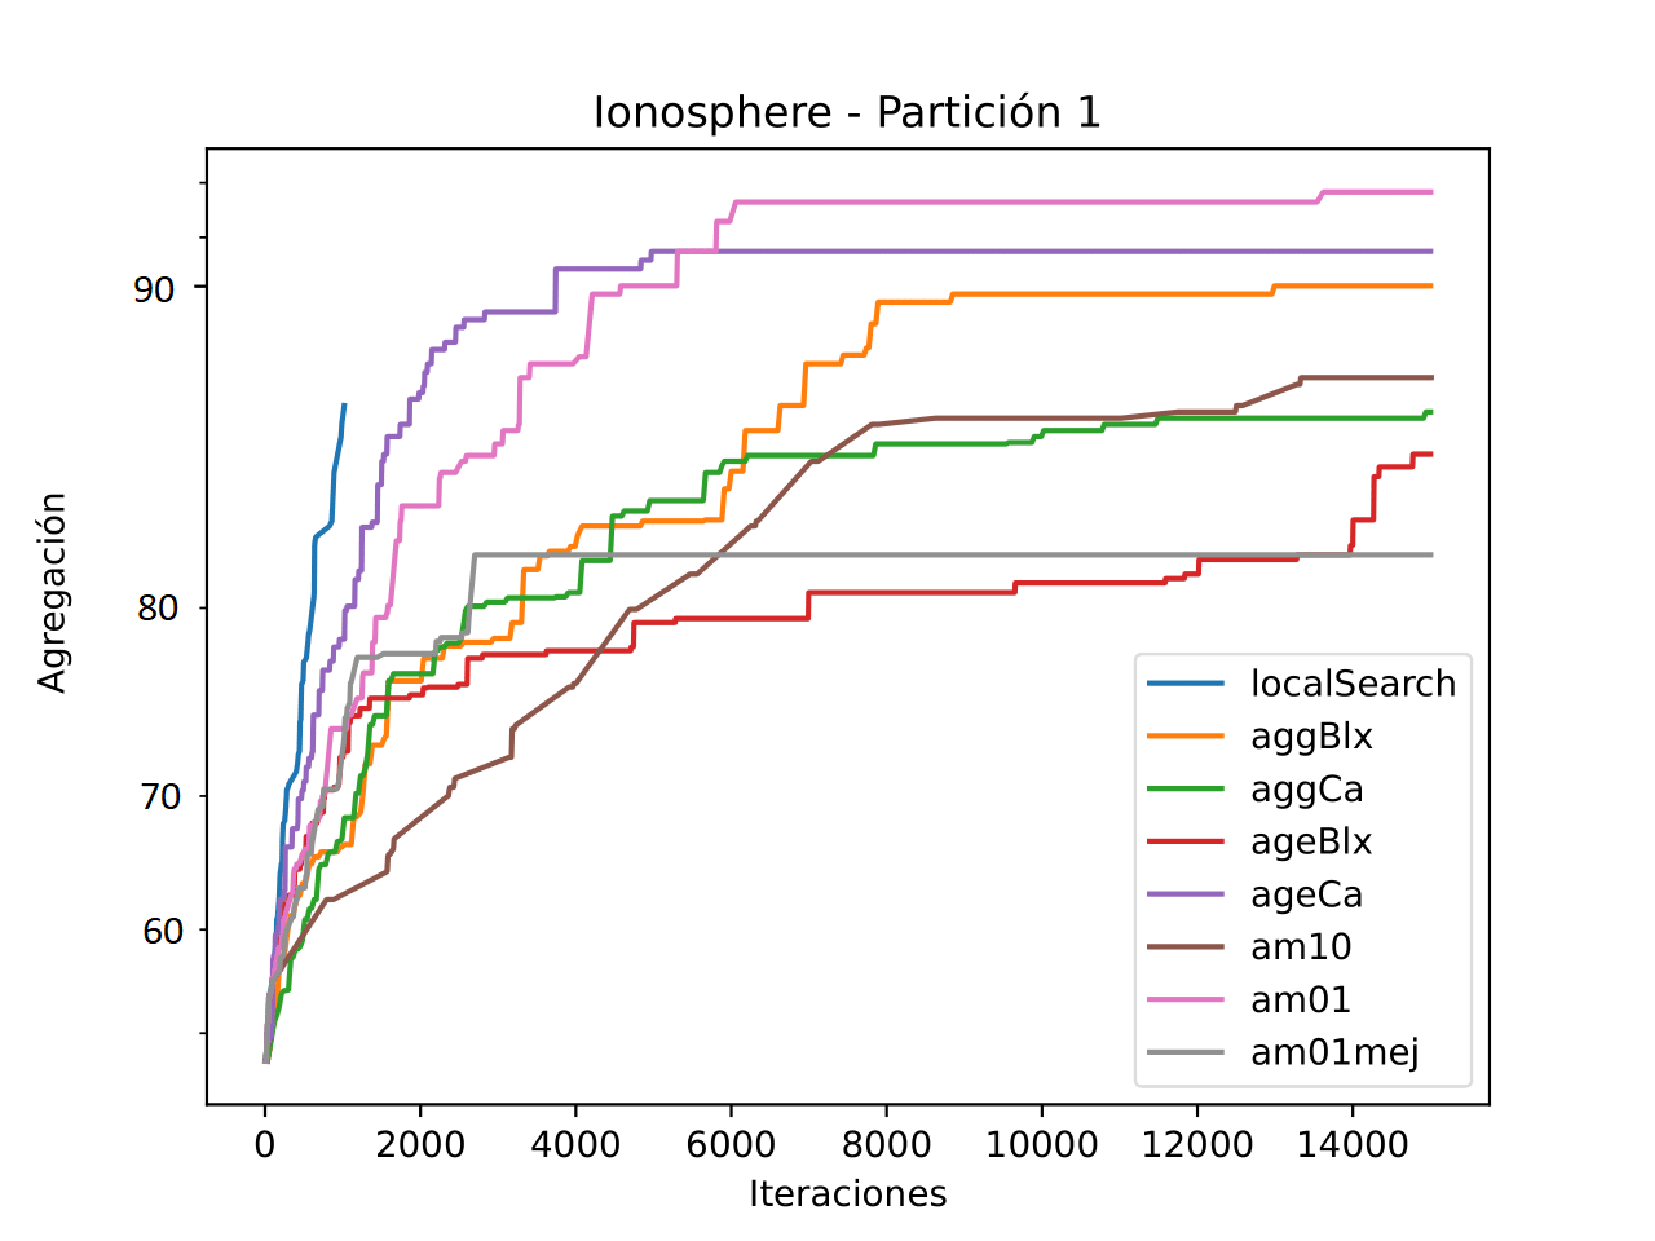
\includegraphics[width=75mm]{../FUENTES/graph/plots/ionosphere1.pdf}}
	\subfigure{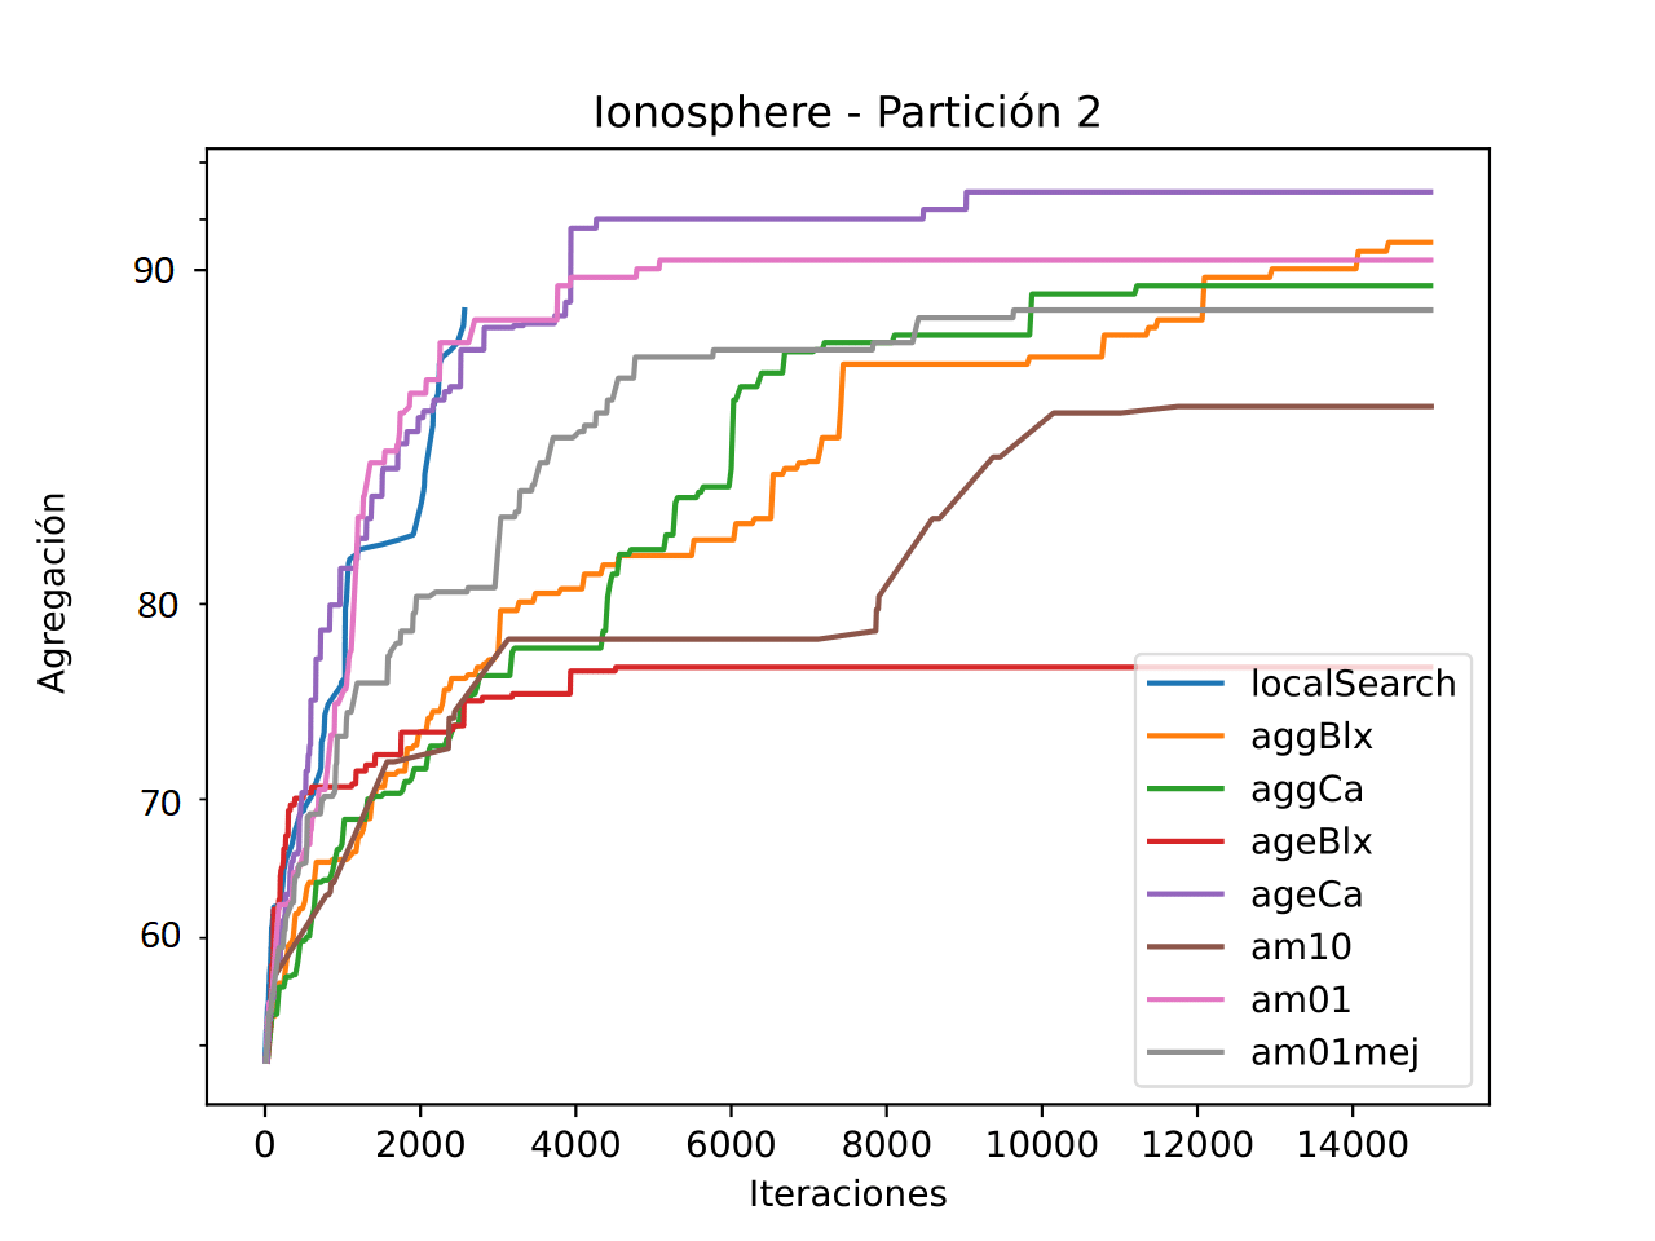
\includegraphics[width=75mm]{../FUENTES/graph/plots/ionosphere2.pdf}}
	\subfigure{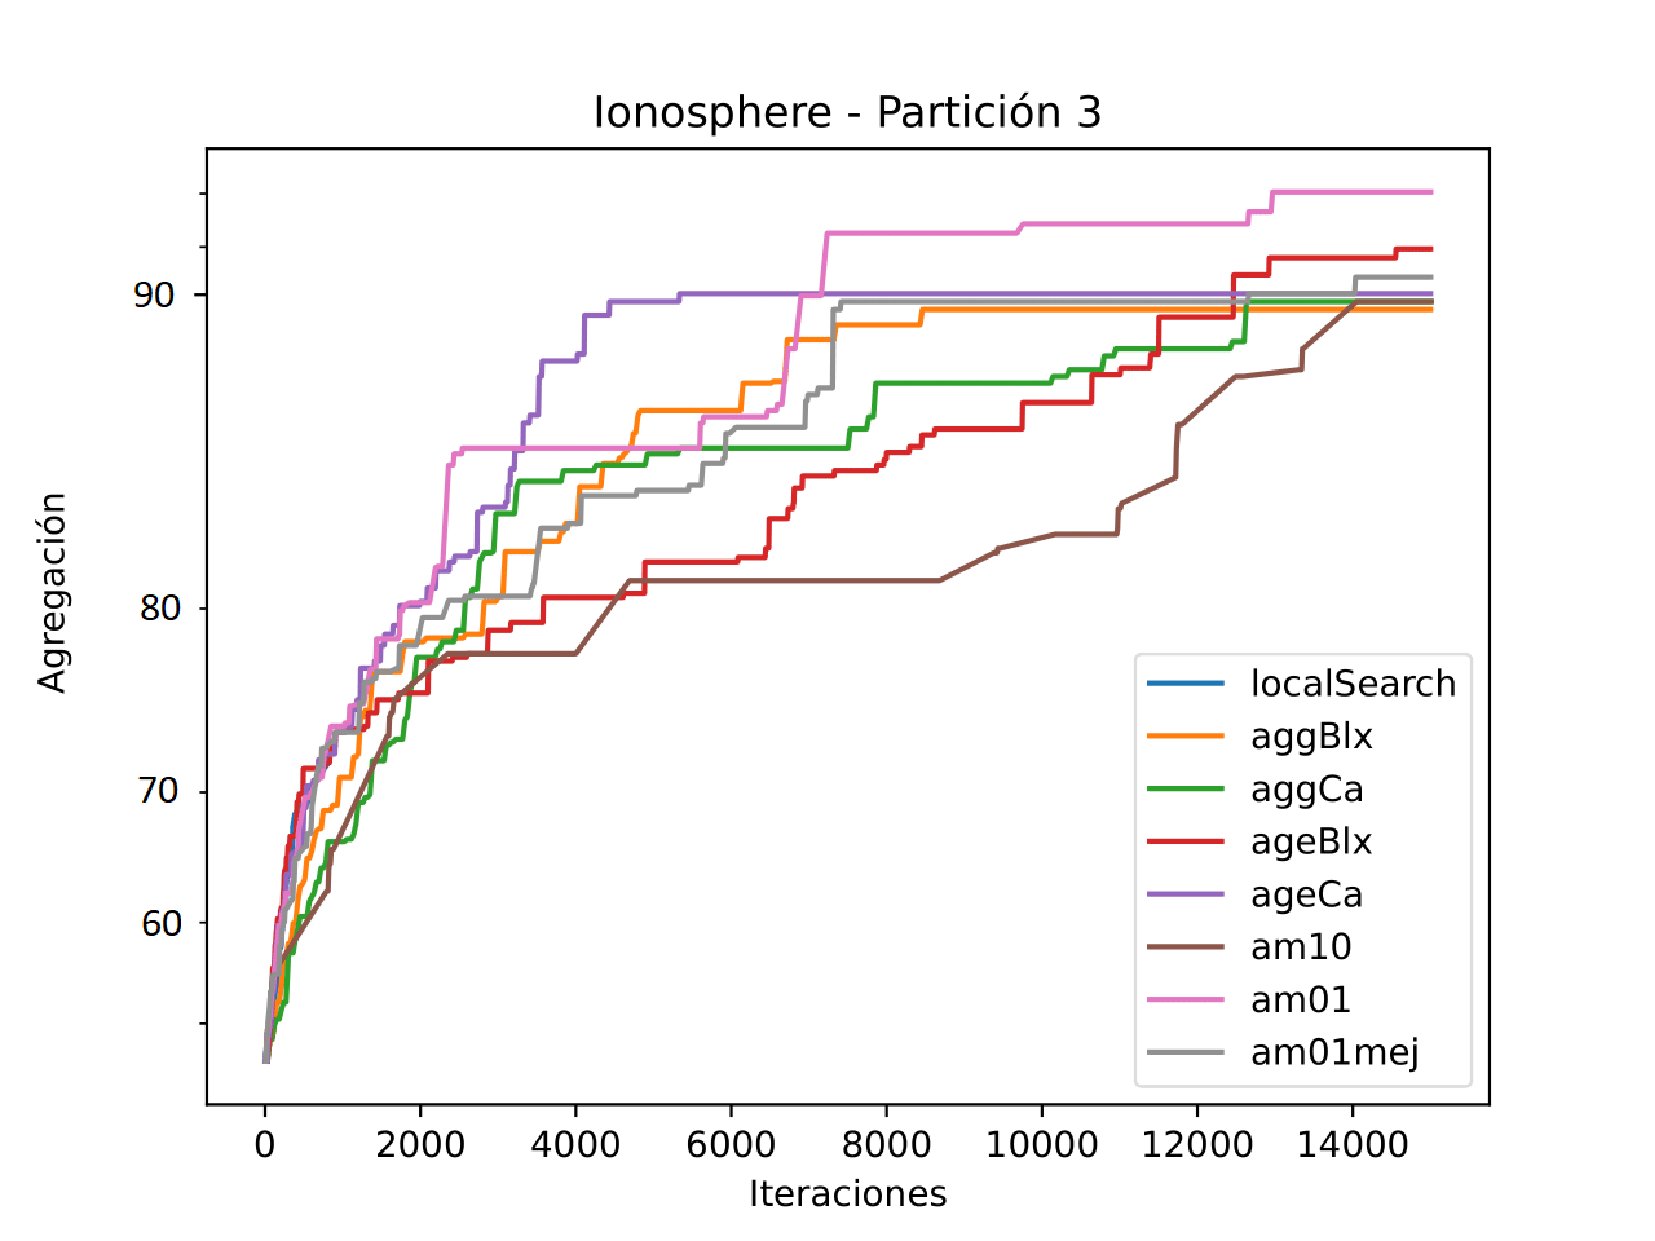
\includegraphics[width=75mm]{../FUENTES/graph/plots/ionosphere3.pdf}}
	\subfigure{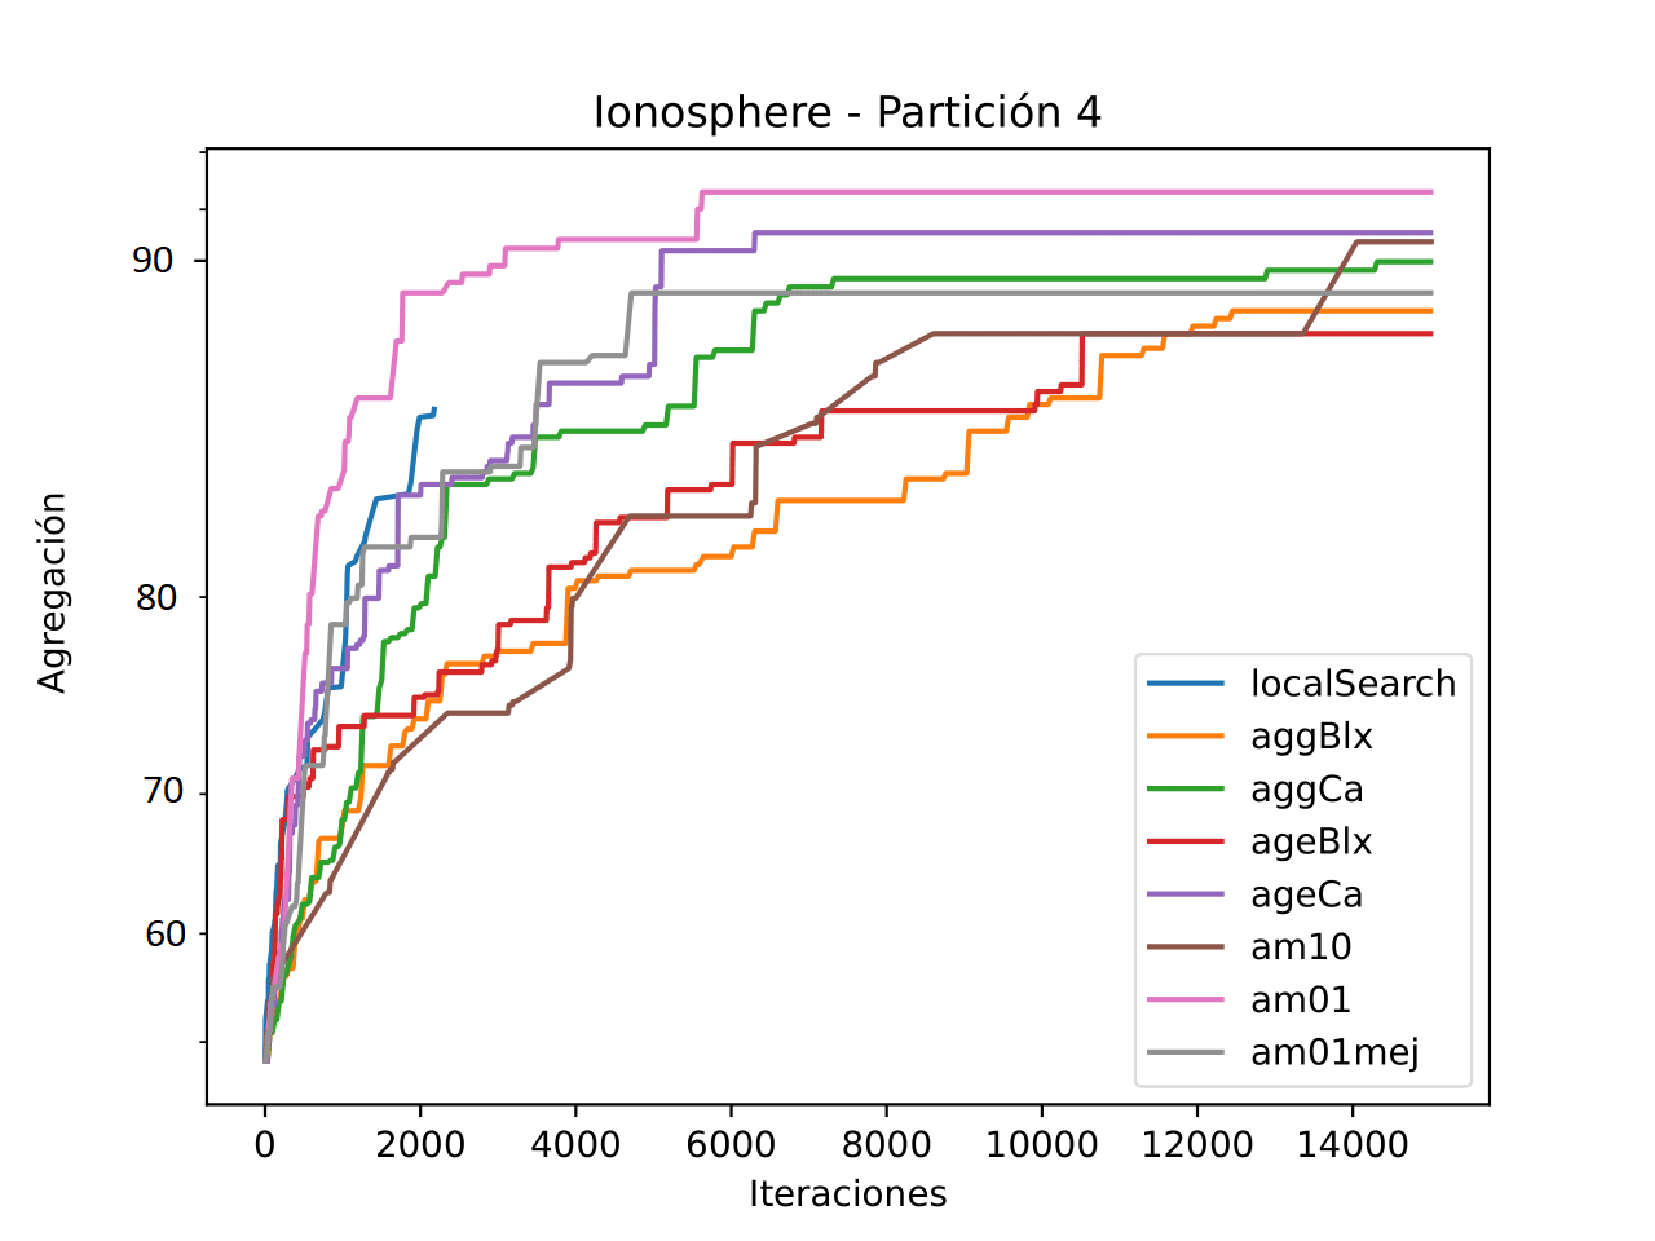
\includegraphics[width=75mm]{../FUENTES/graph/plots/ionosphere4.pdf}}
	\subfigure{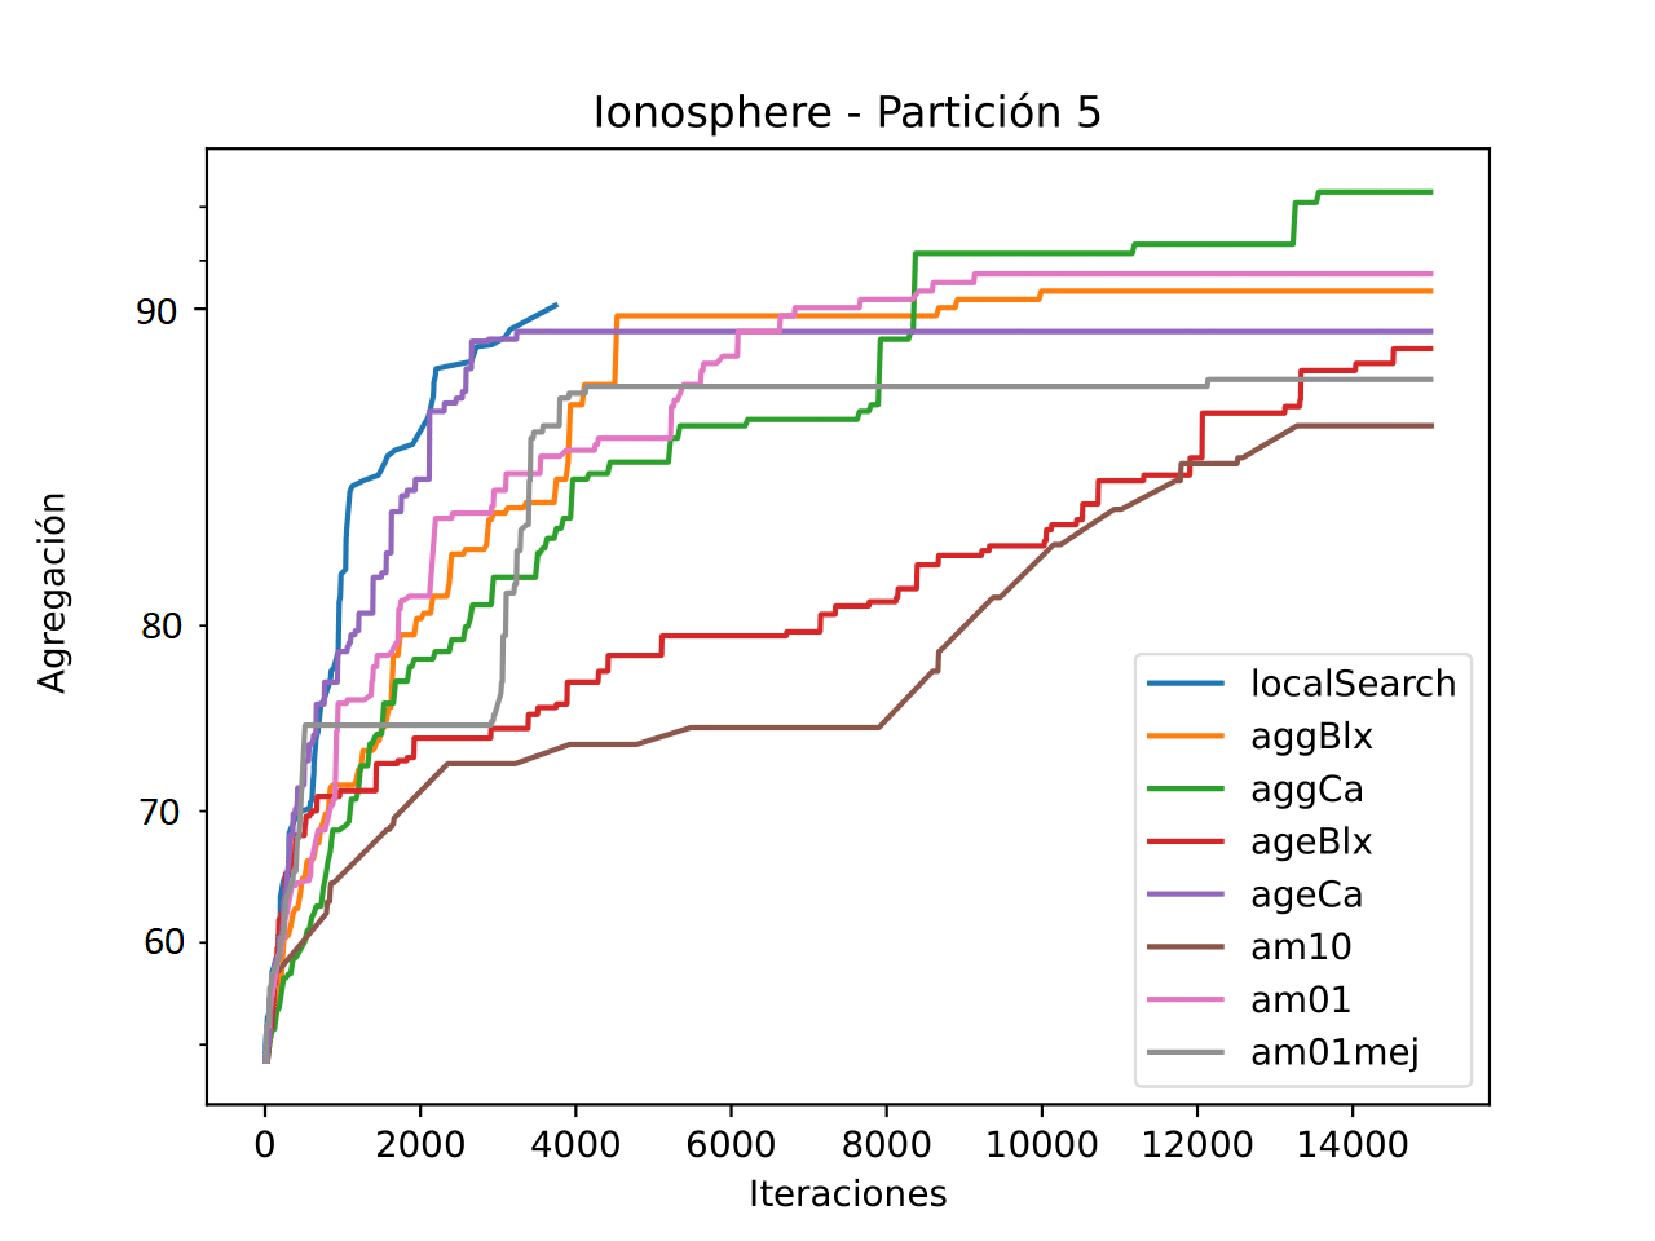
\includegraphics[width=75mm]{../FUENTES/graph/plots/ionosphere5.pdf}}
	\caption{Gráficas de la agregación respecto al número de iteraciones con los datos de train de Ionosphere}
\end{figure}

\begin{figure}[H]
	\centering
	\subfigure{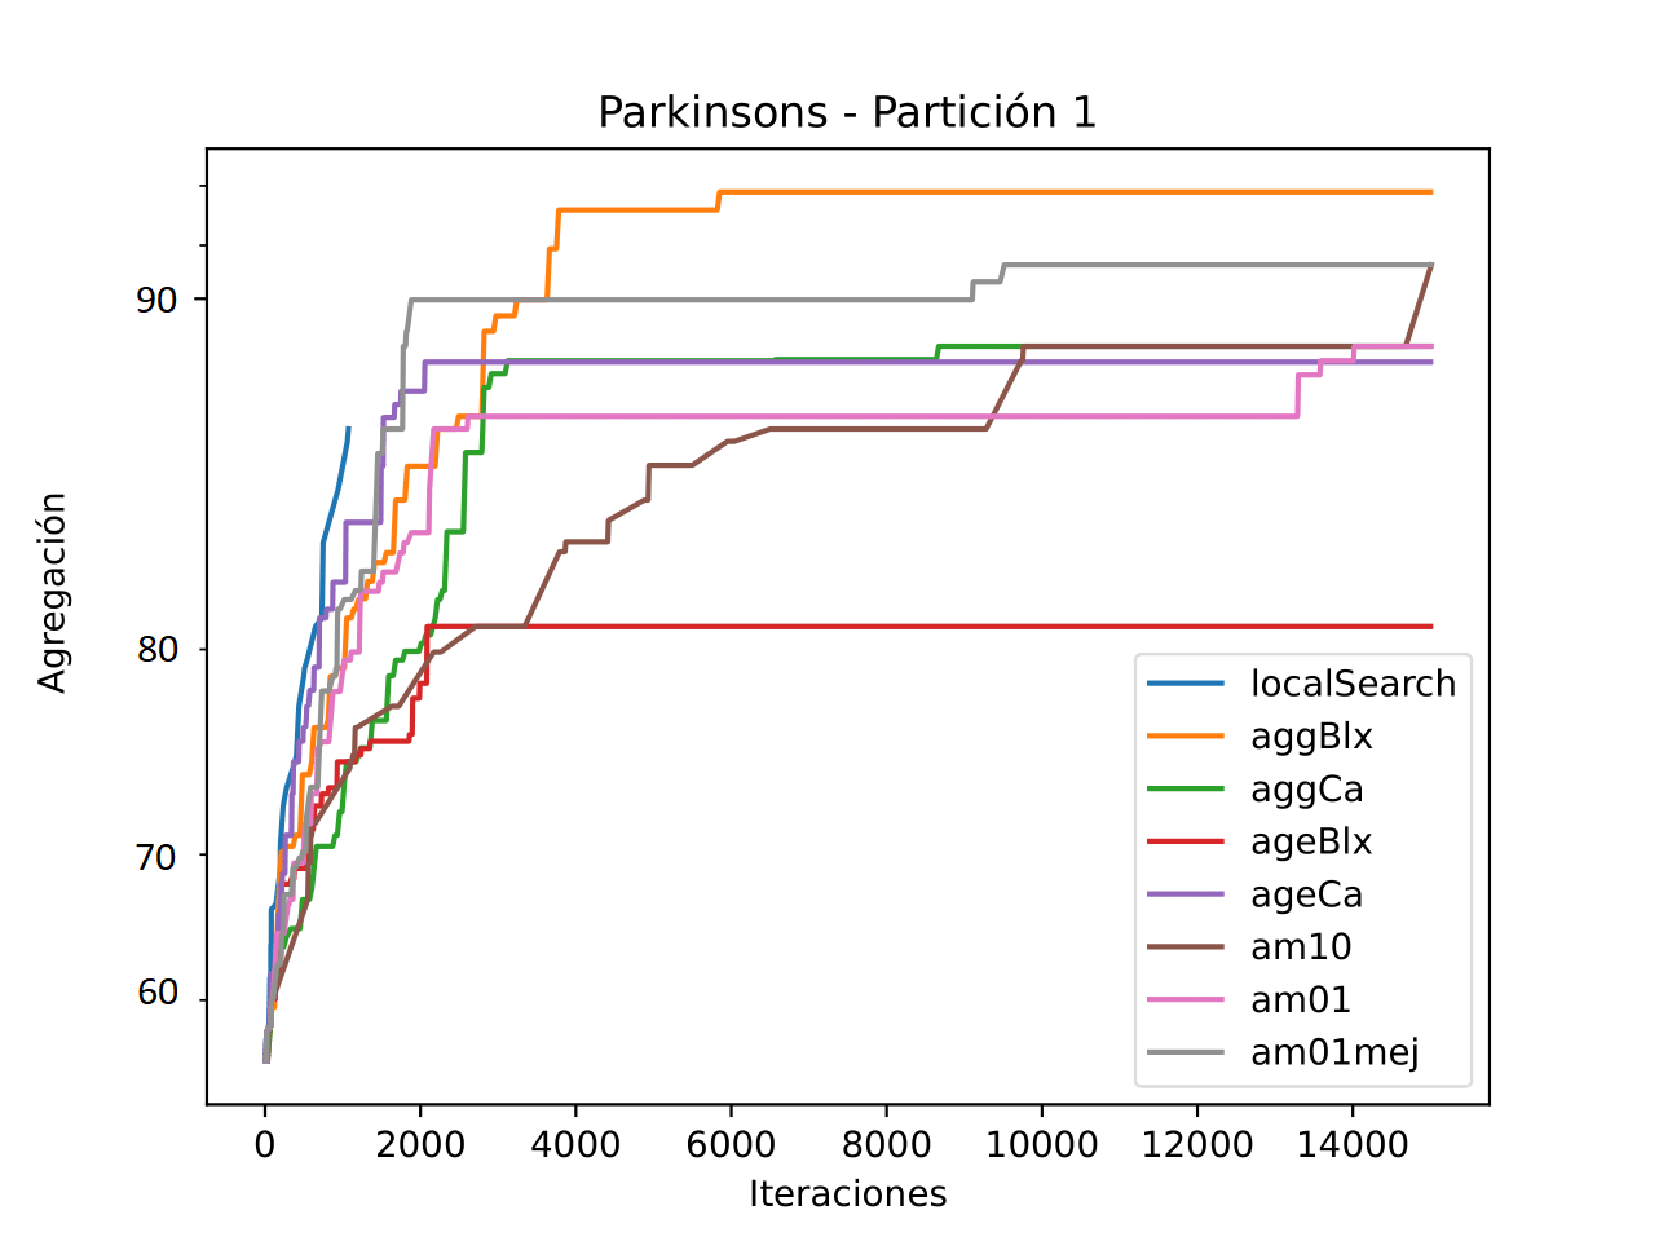
\includegraphics[width=75mm]{../FUENTES/graph/plots/parkinsons1.pdf}}
	\subfigure{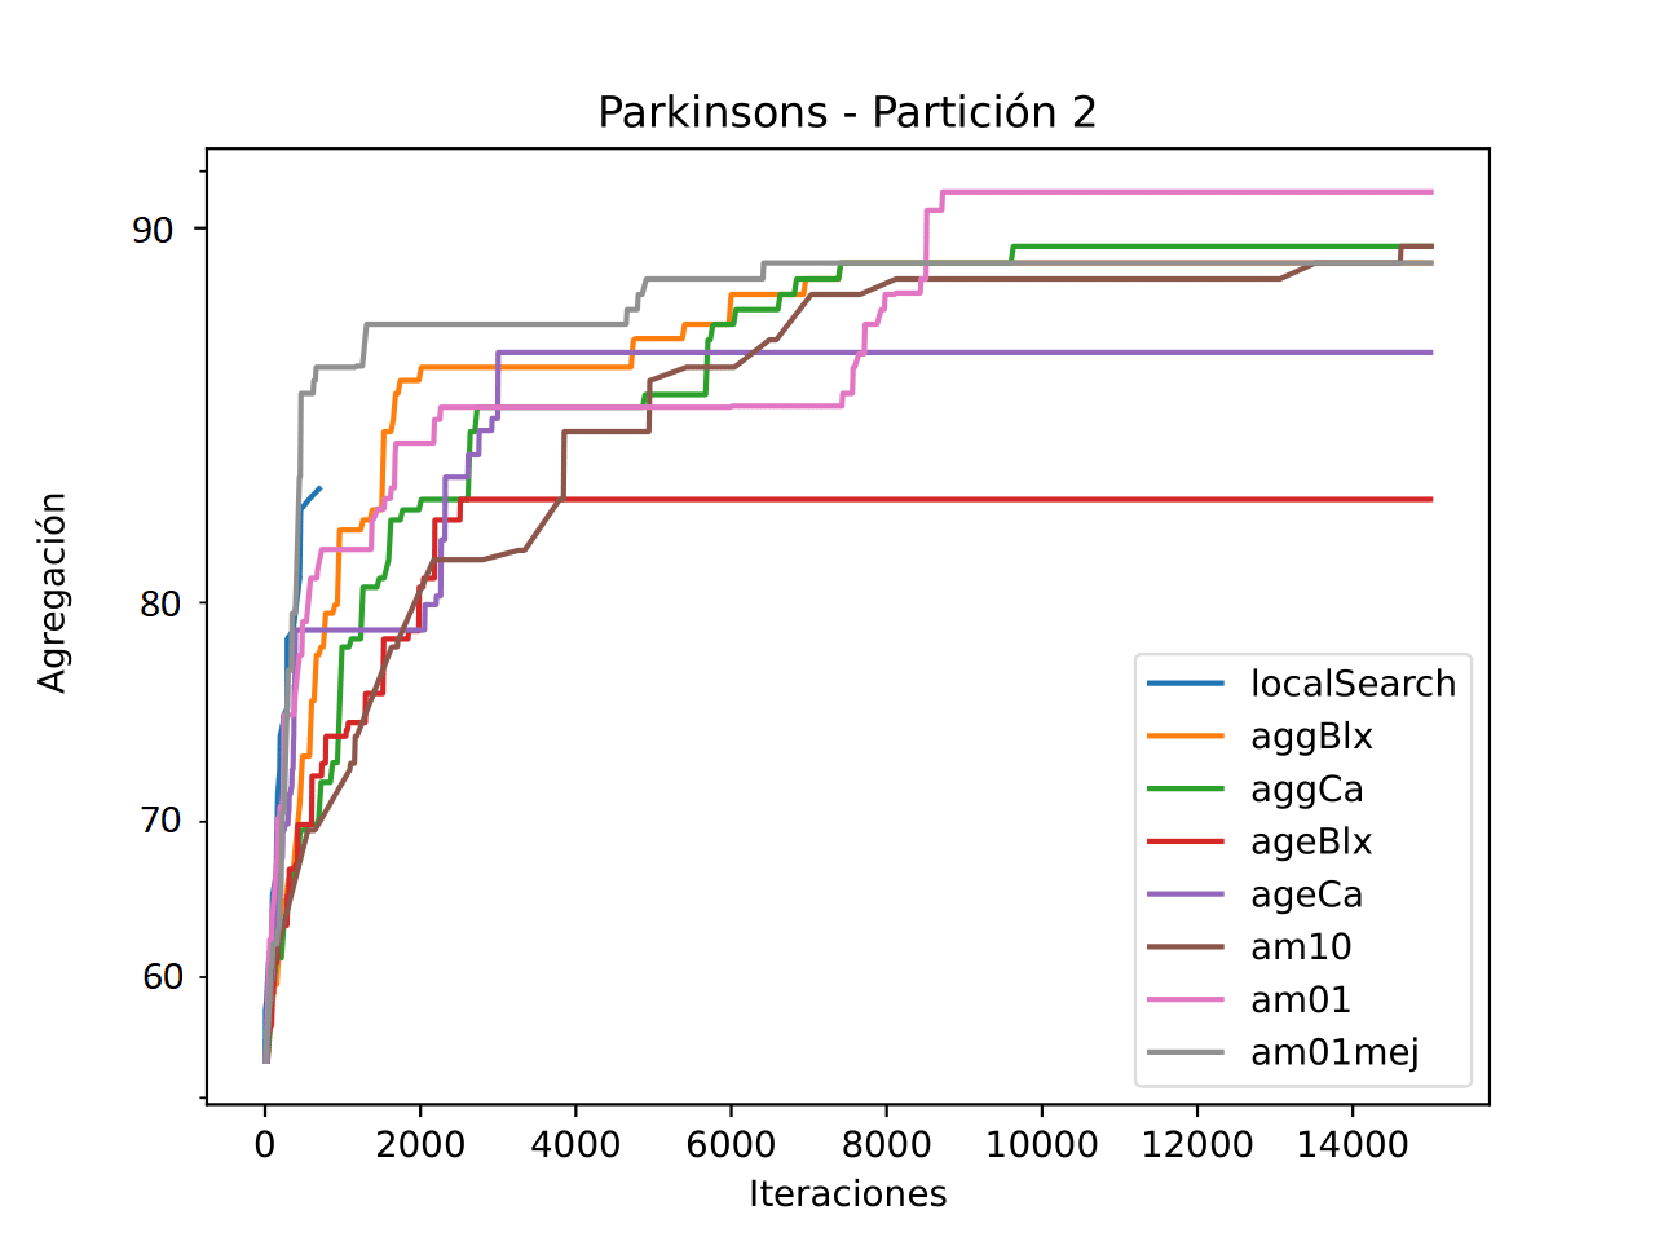
\includegraphics[width=75mm]{../FUENTES/graph/plots/parkinsons2.pdf}}
	\subfigure{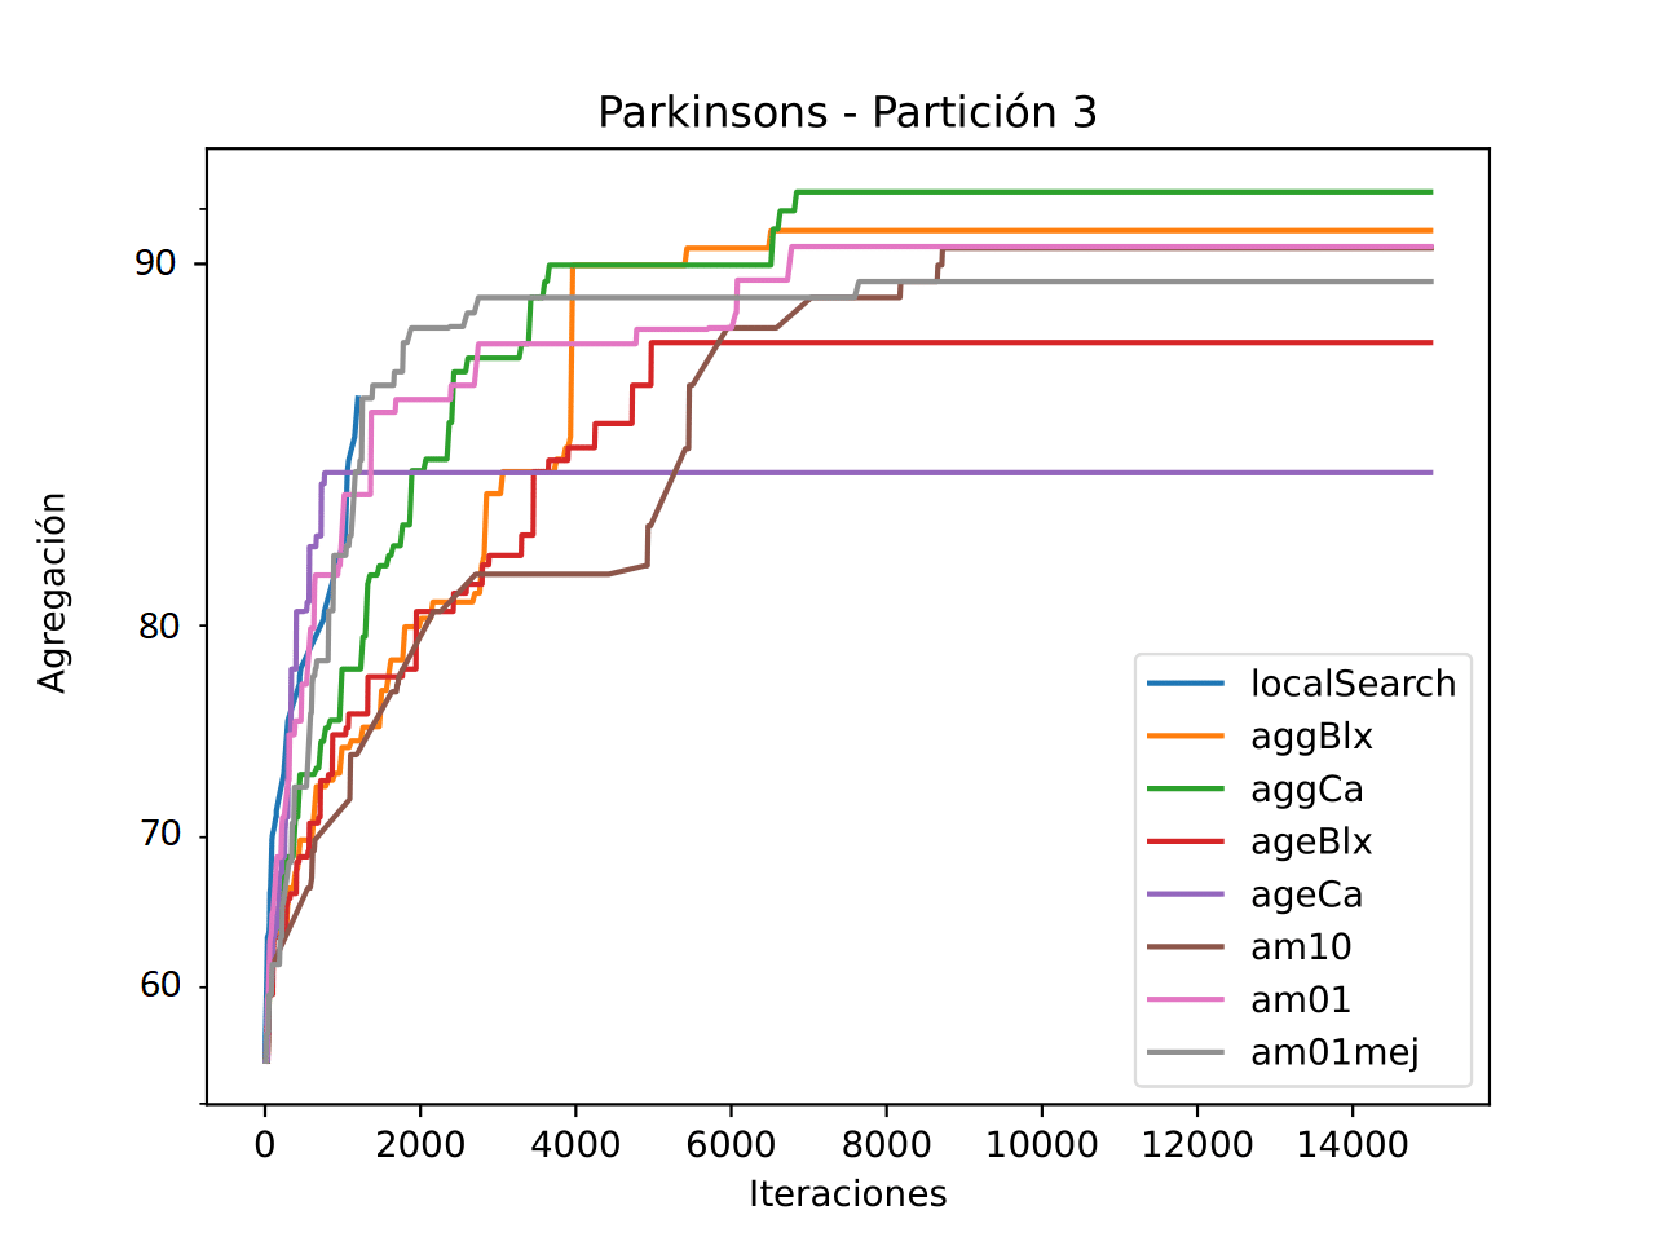
\includegraphics[width=75mm]{../FUENTES/graph/plots/parkinsons3.pdf}}
	\subfigure{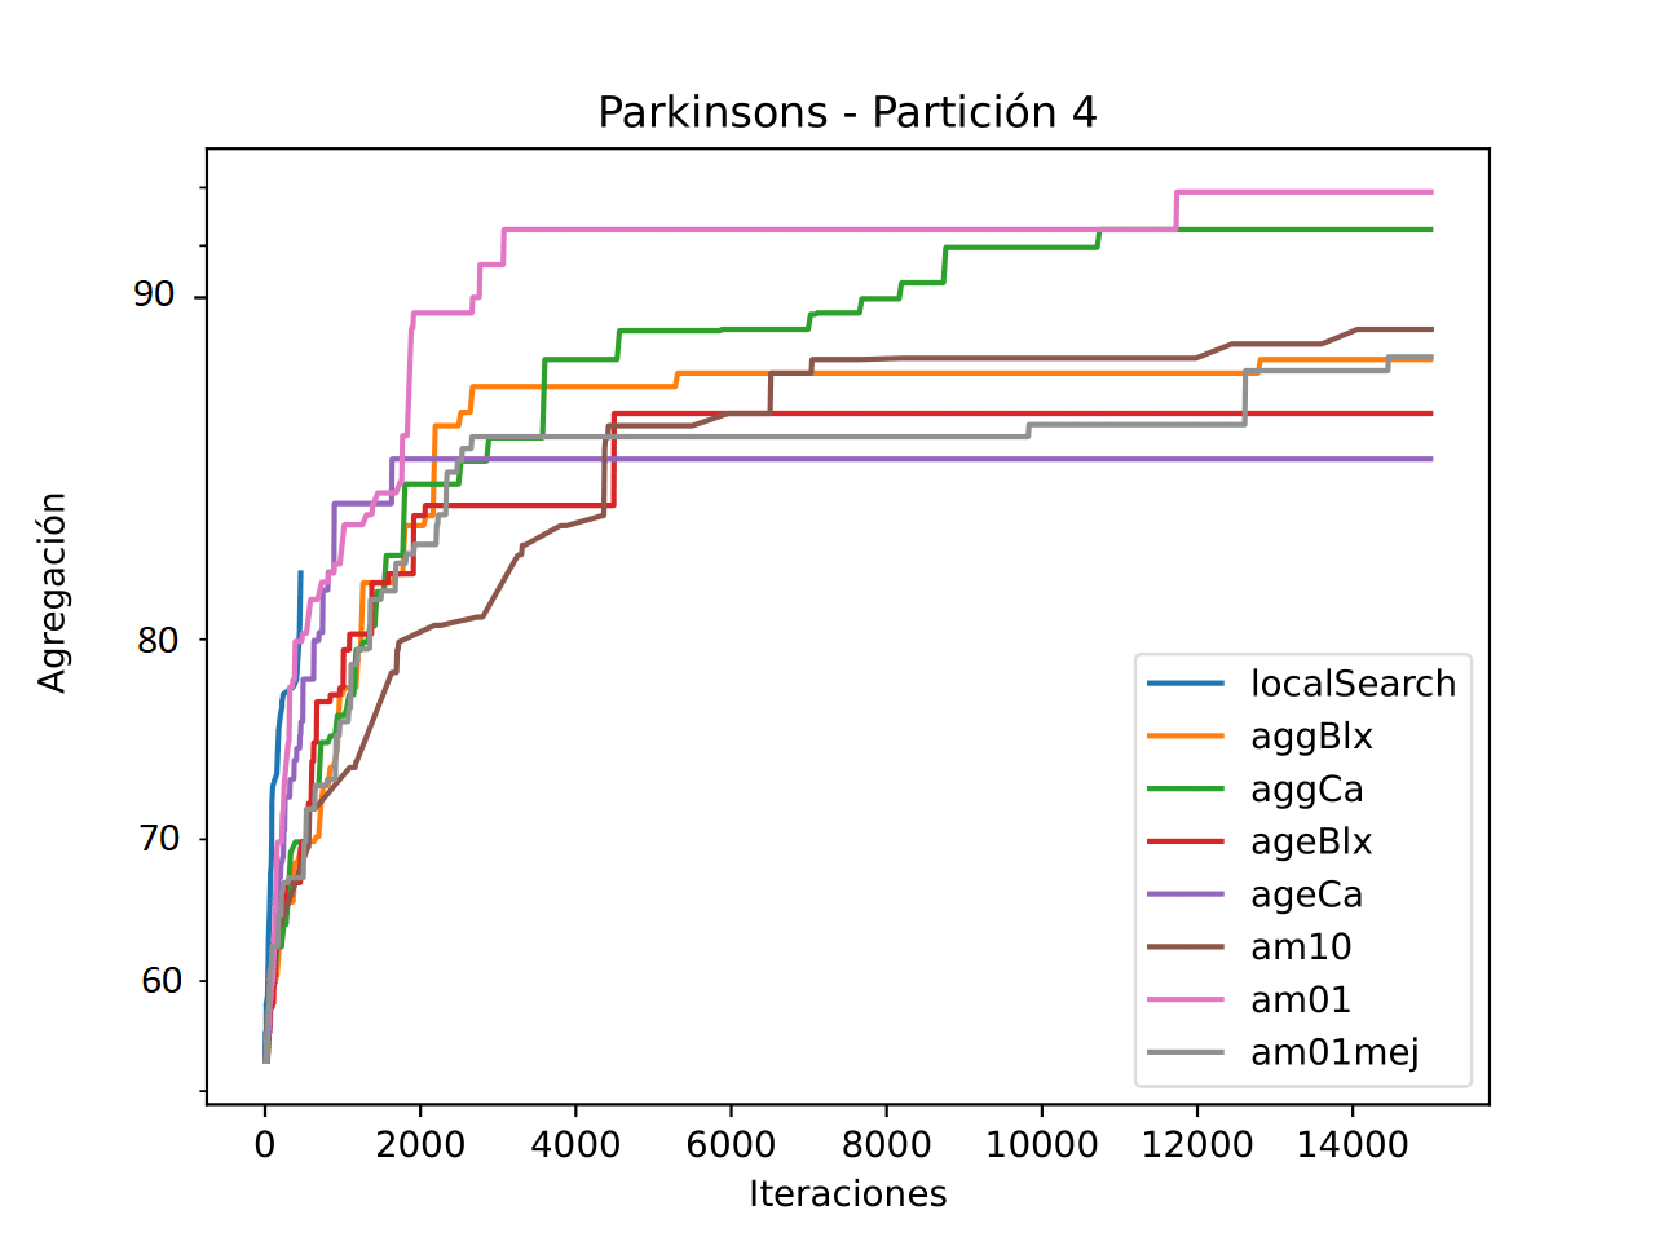
\includegraphics[width=75mm]{../FUENTES/graph/plots/parkinsons4.pdf}}
	\subfigure{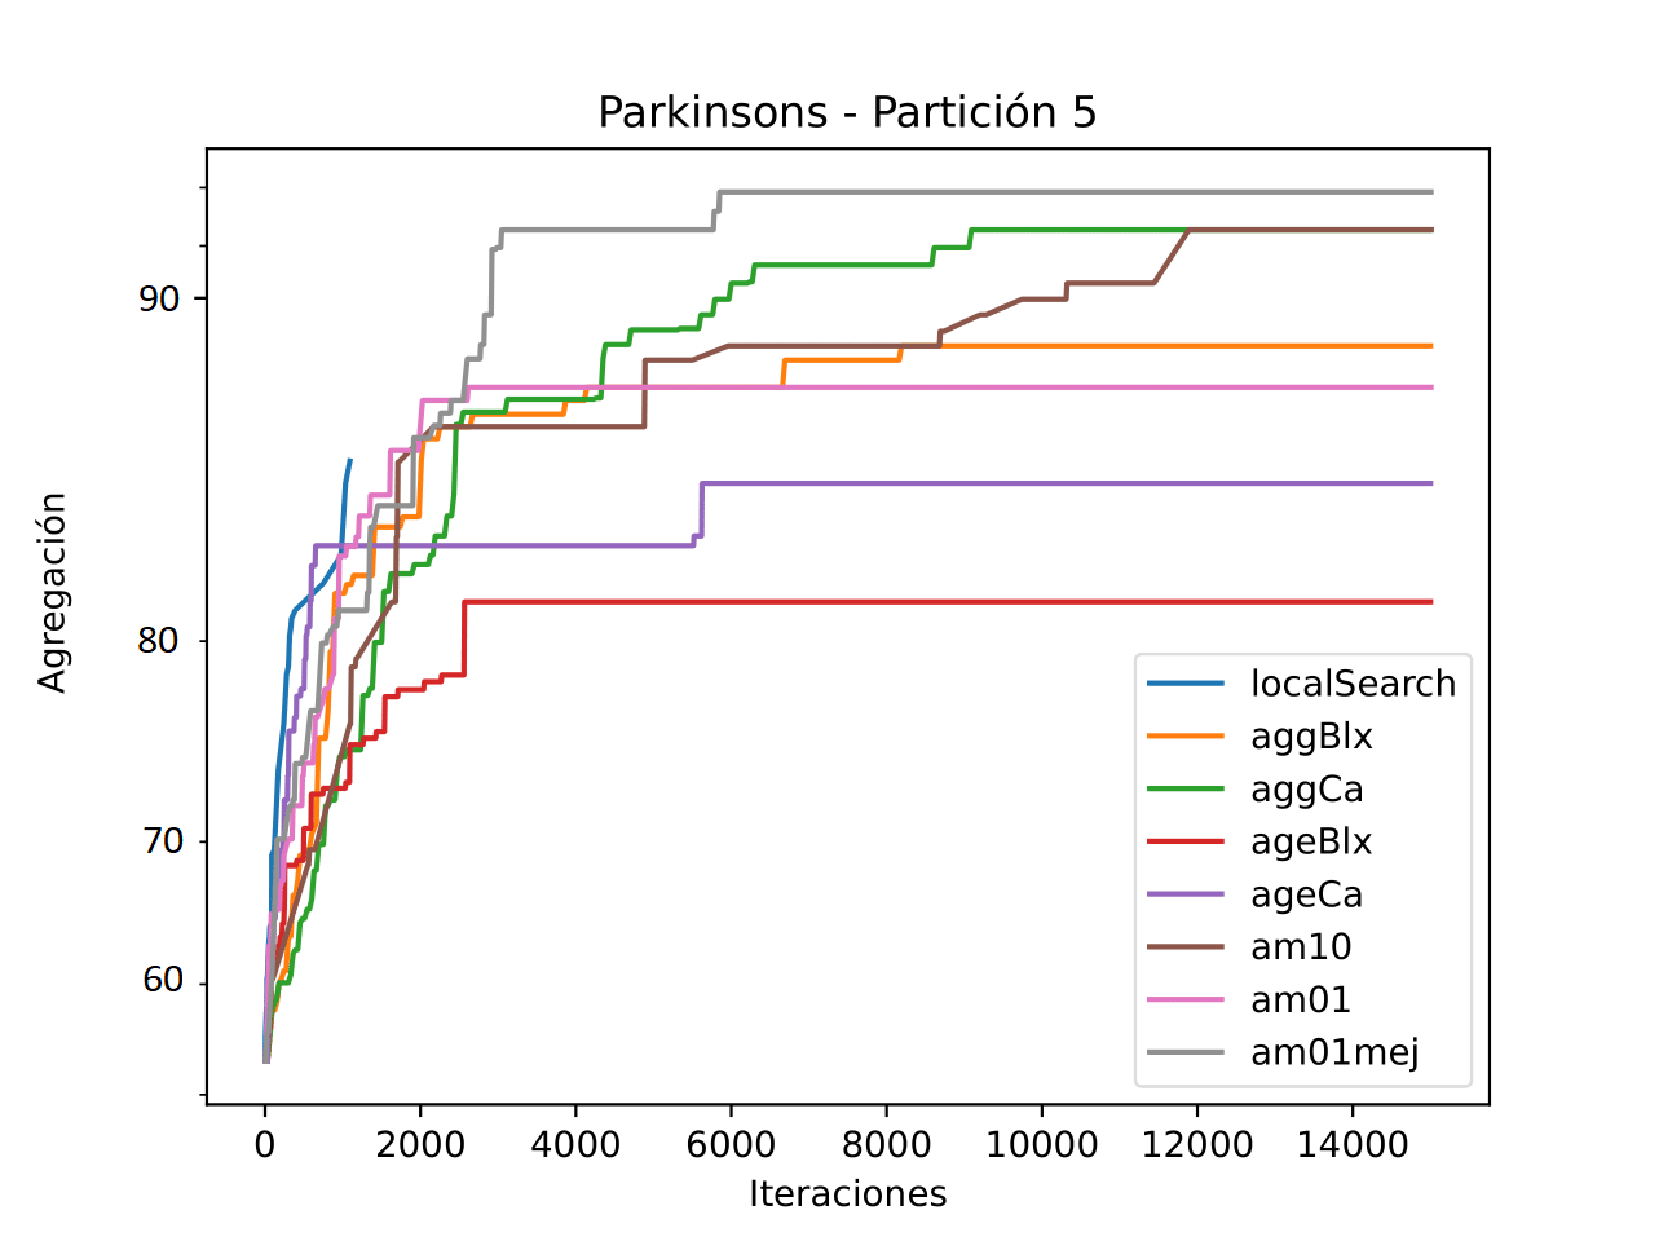
\includegraphics[width=75mm]{../FUENTES/graph/plots/parkinsons5.pdf}}
	\caption{Gráficas de la agregación respecto al número de iteraciones con los datos de train de Parkinsons}
\end{figure}

\begin{figure}[H]
	\centering
	\subfigure{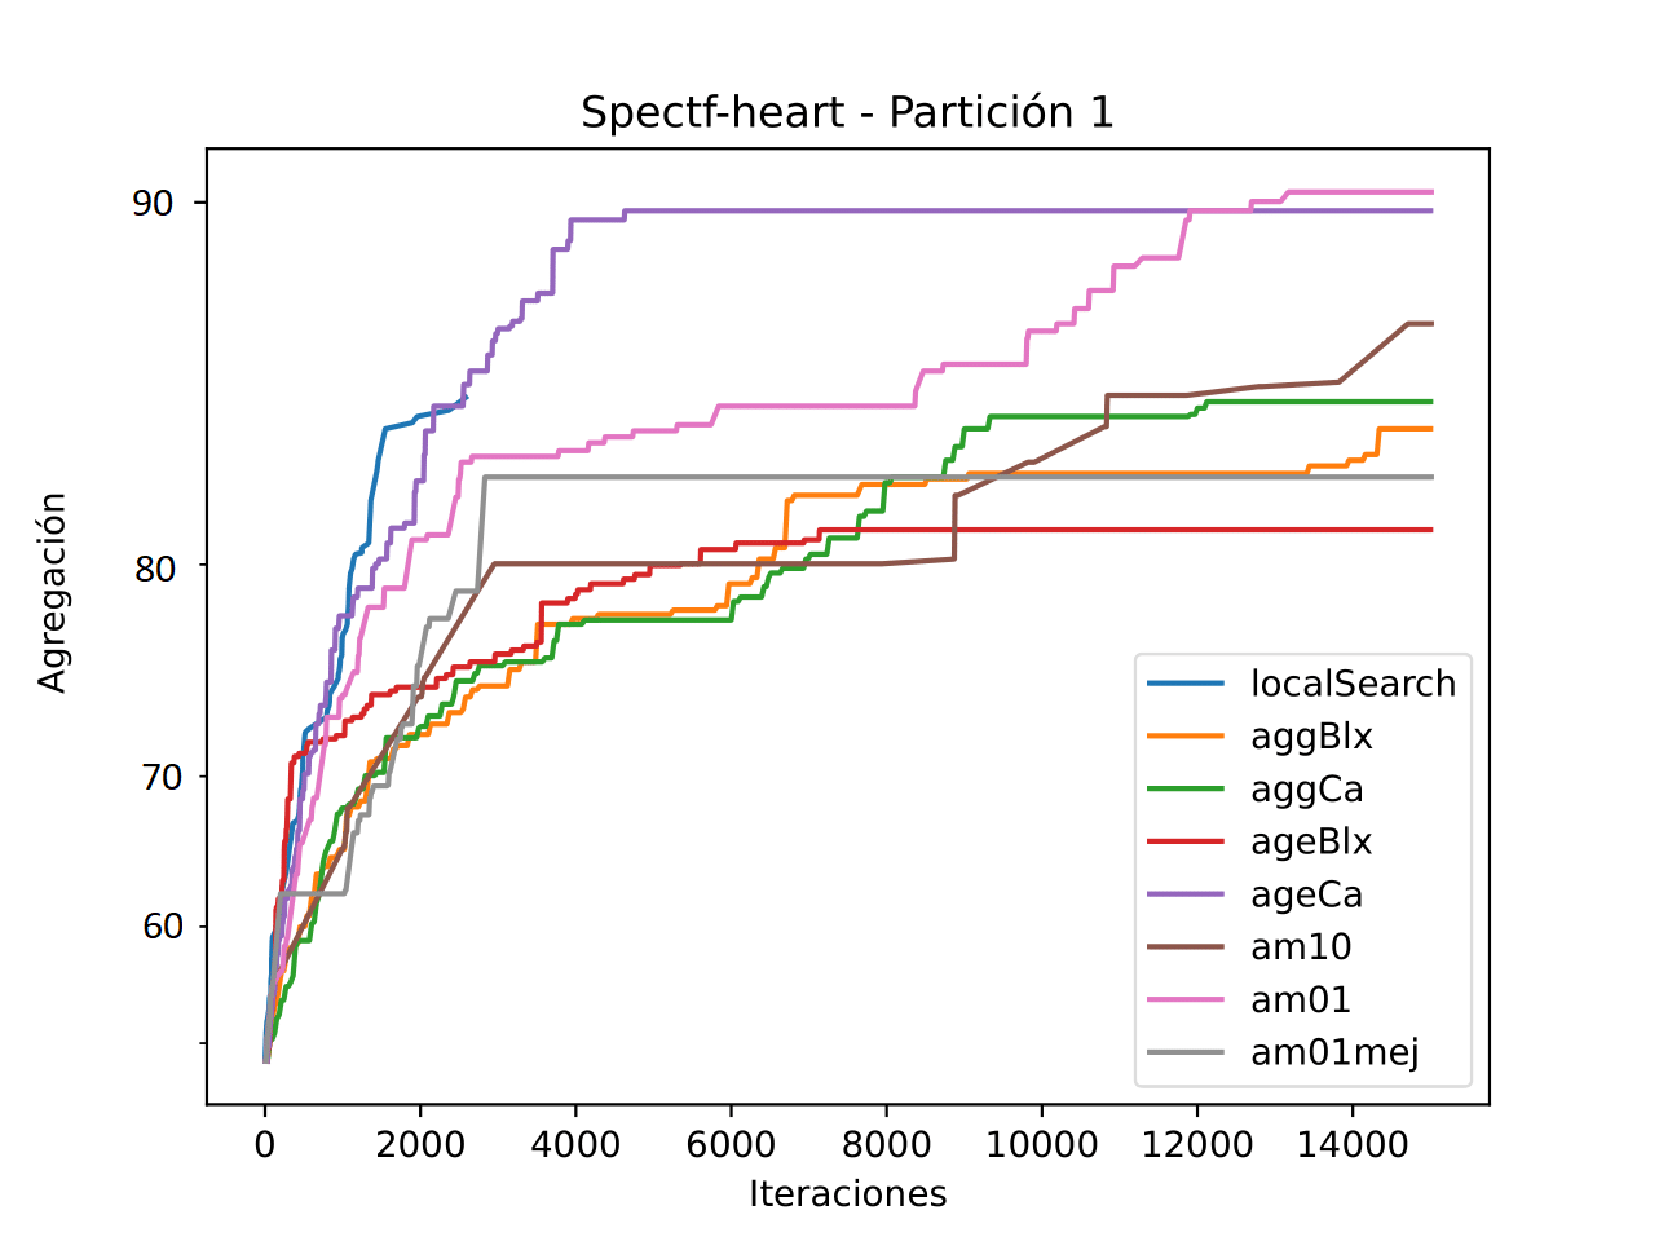
\includegraphics[width=75mm]{../FUENTES/graph/plots/spectf-heart1.pdf}}
	\subfigure{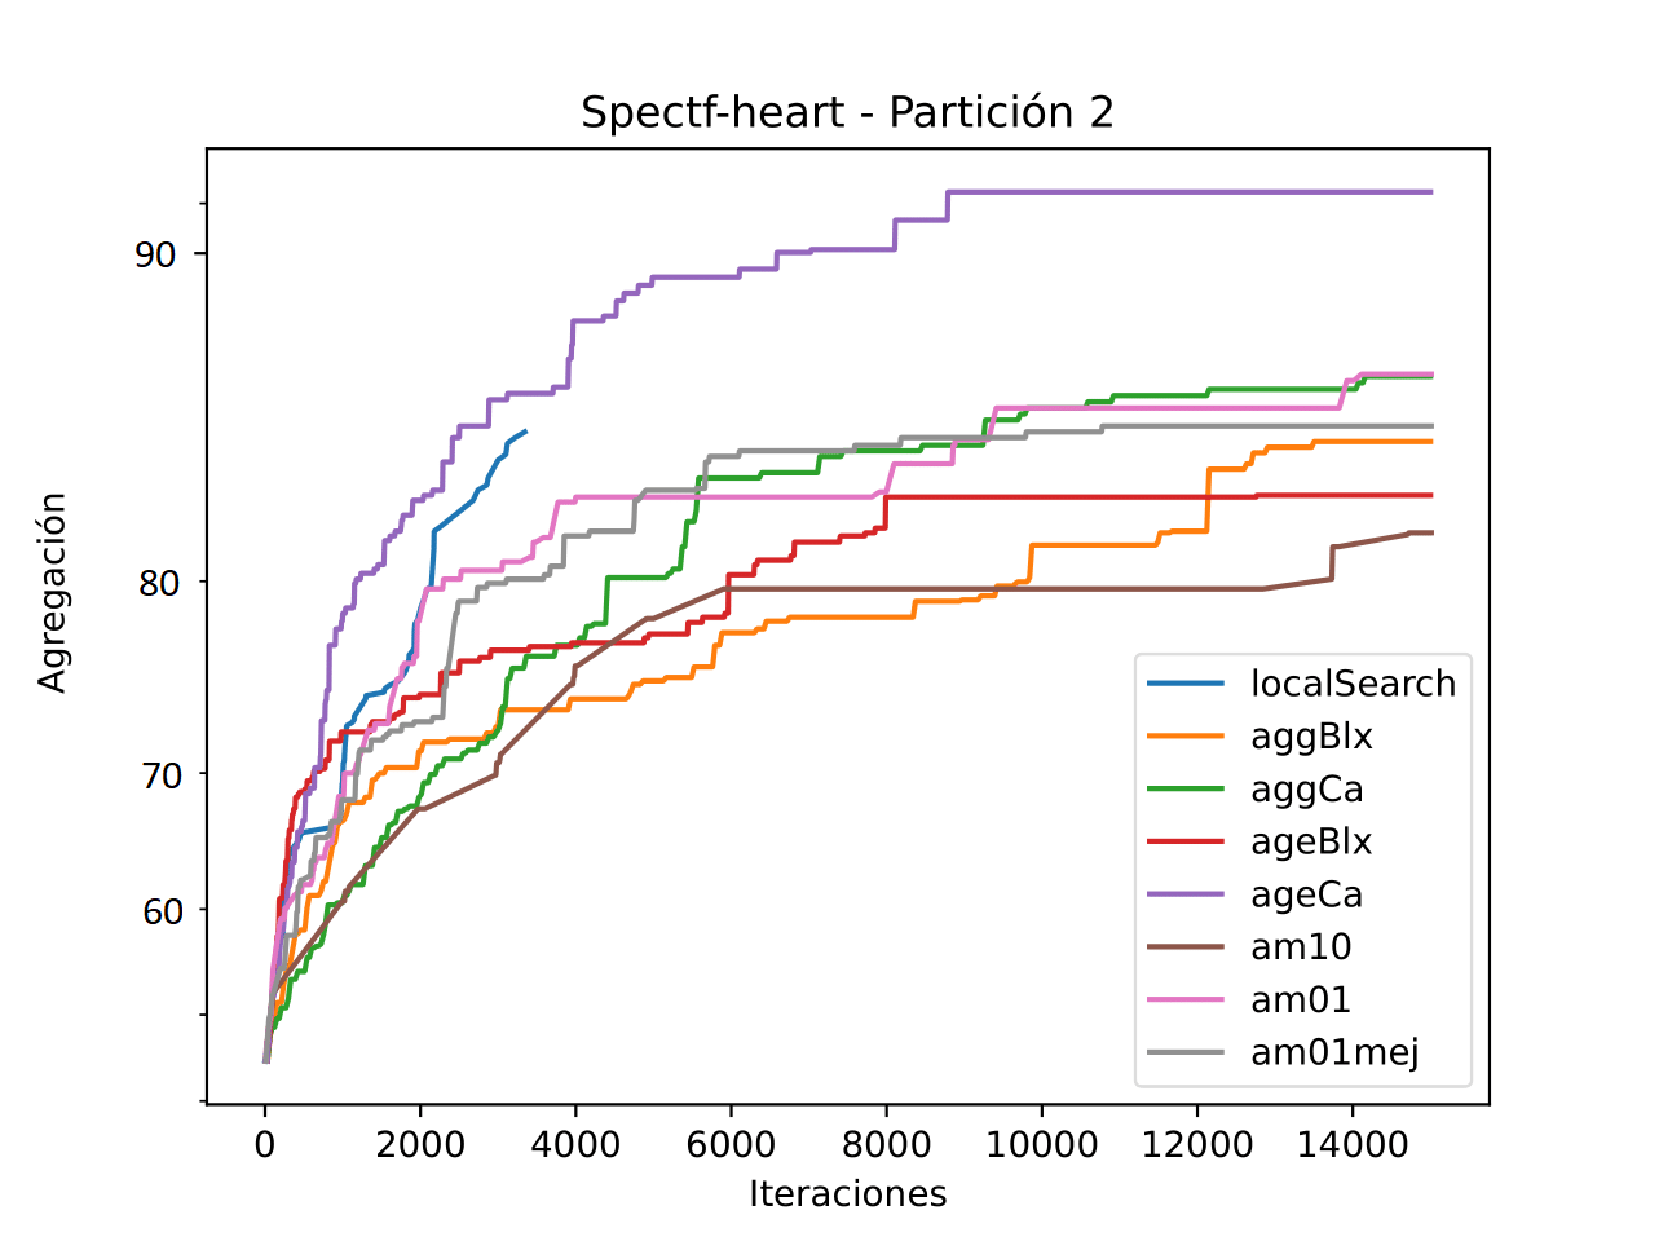
\includegraphics[width=75mm]{../FUENTES/graph/plots/spectf-heart2.pdf}}
	\subfigure{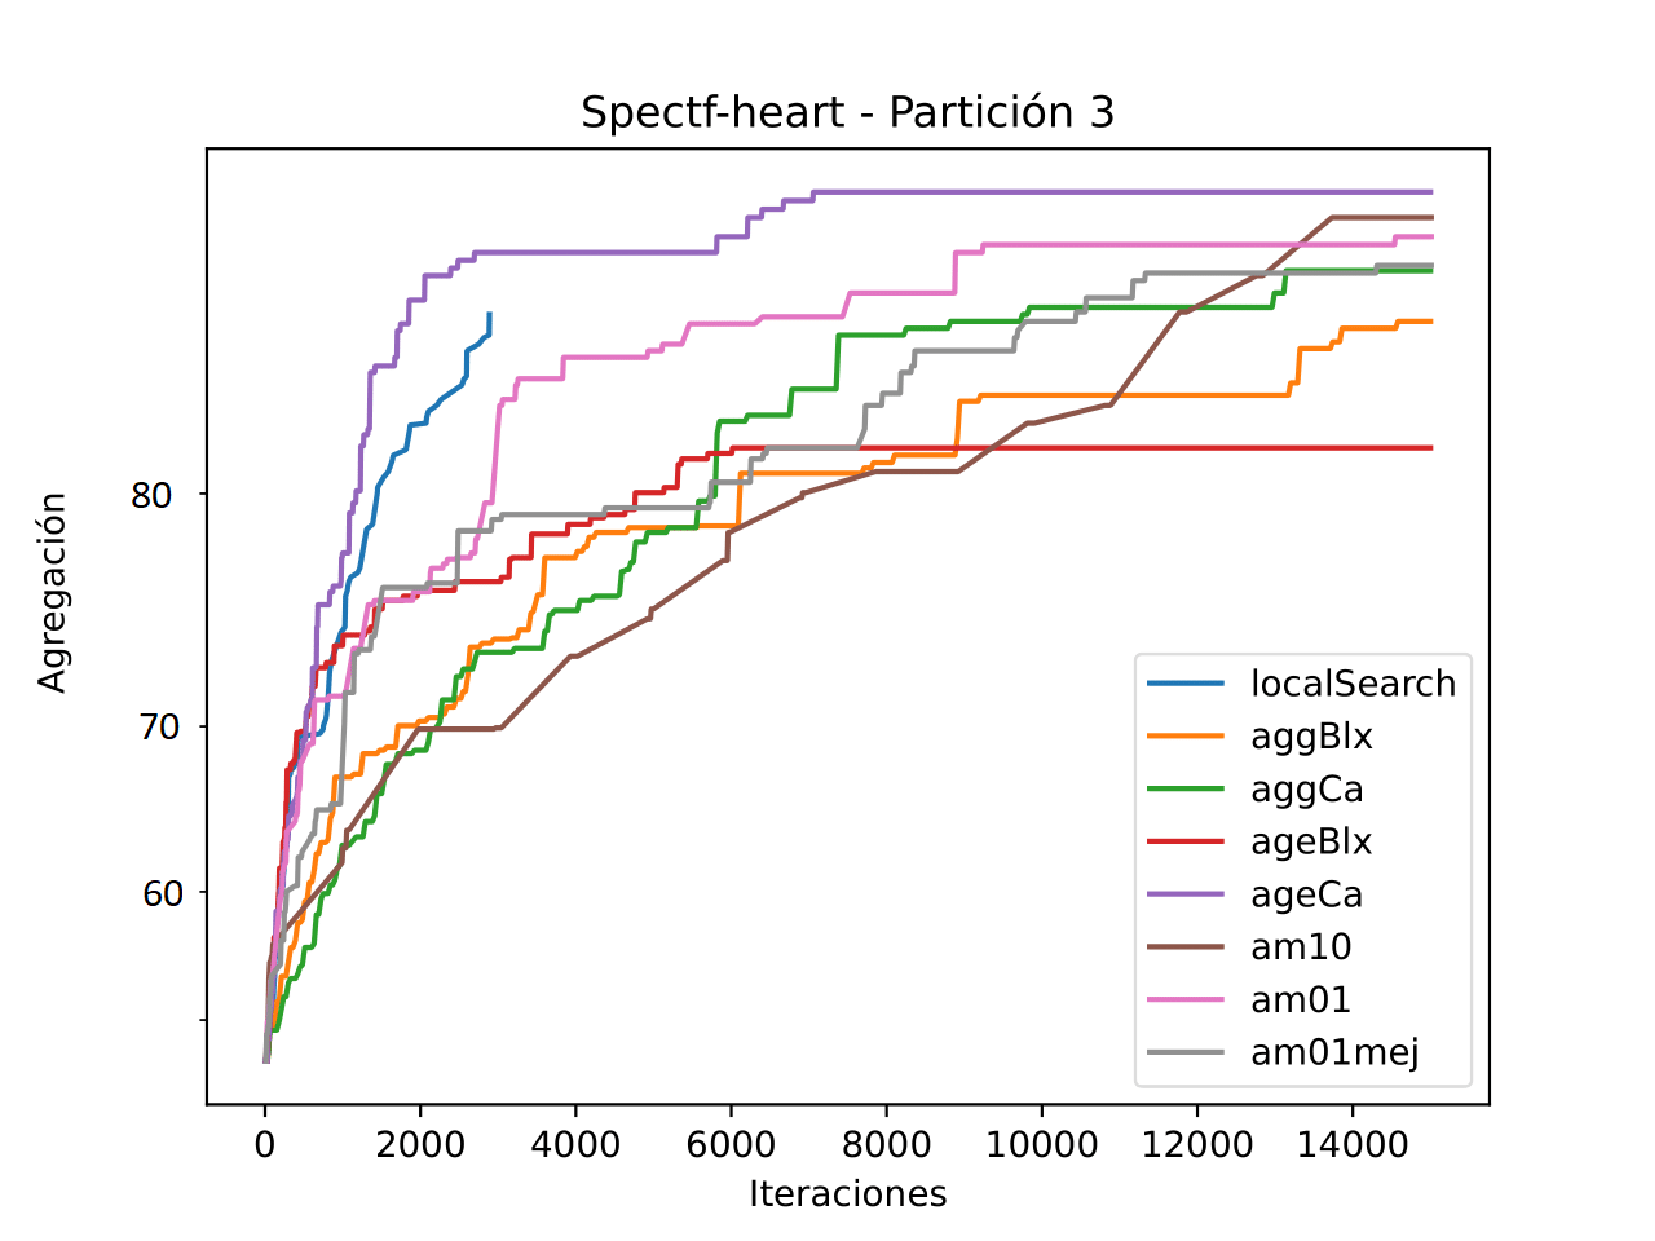
\includegraphics[width=75mm]{../FUENTES/graph/plots/spectf-heart3.pdf}}
	\subfigure{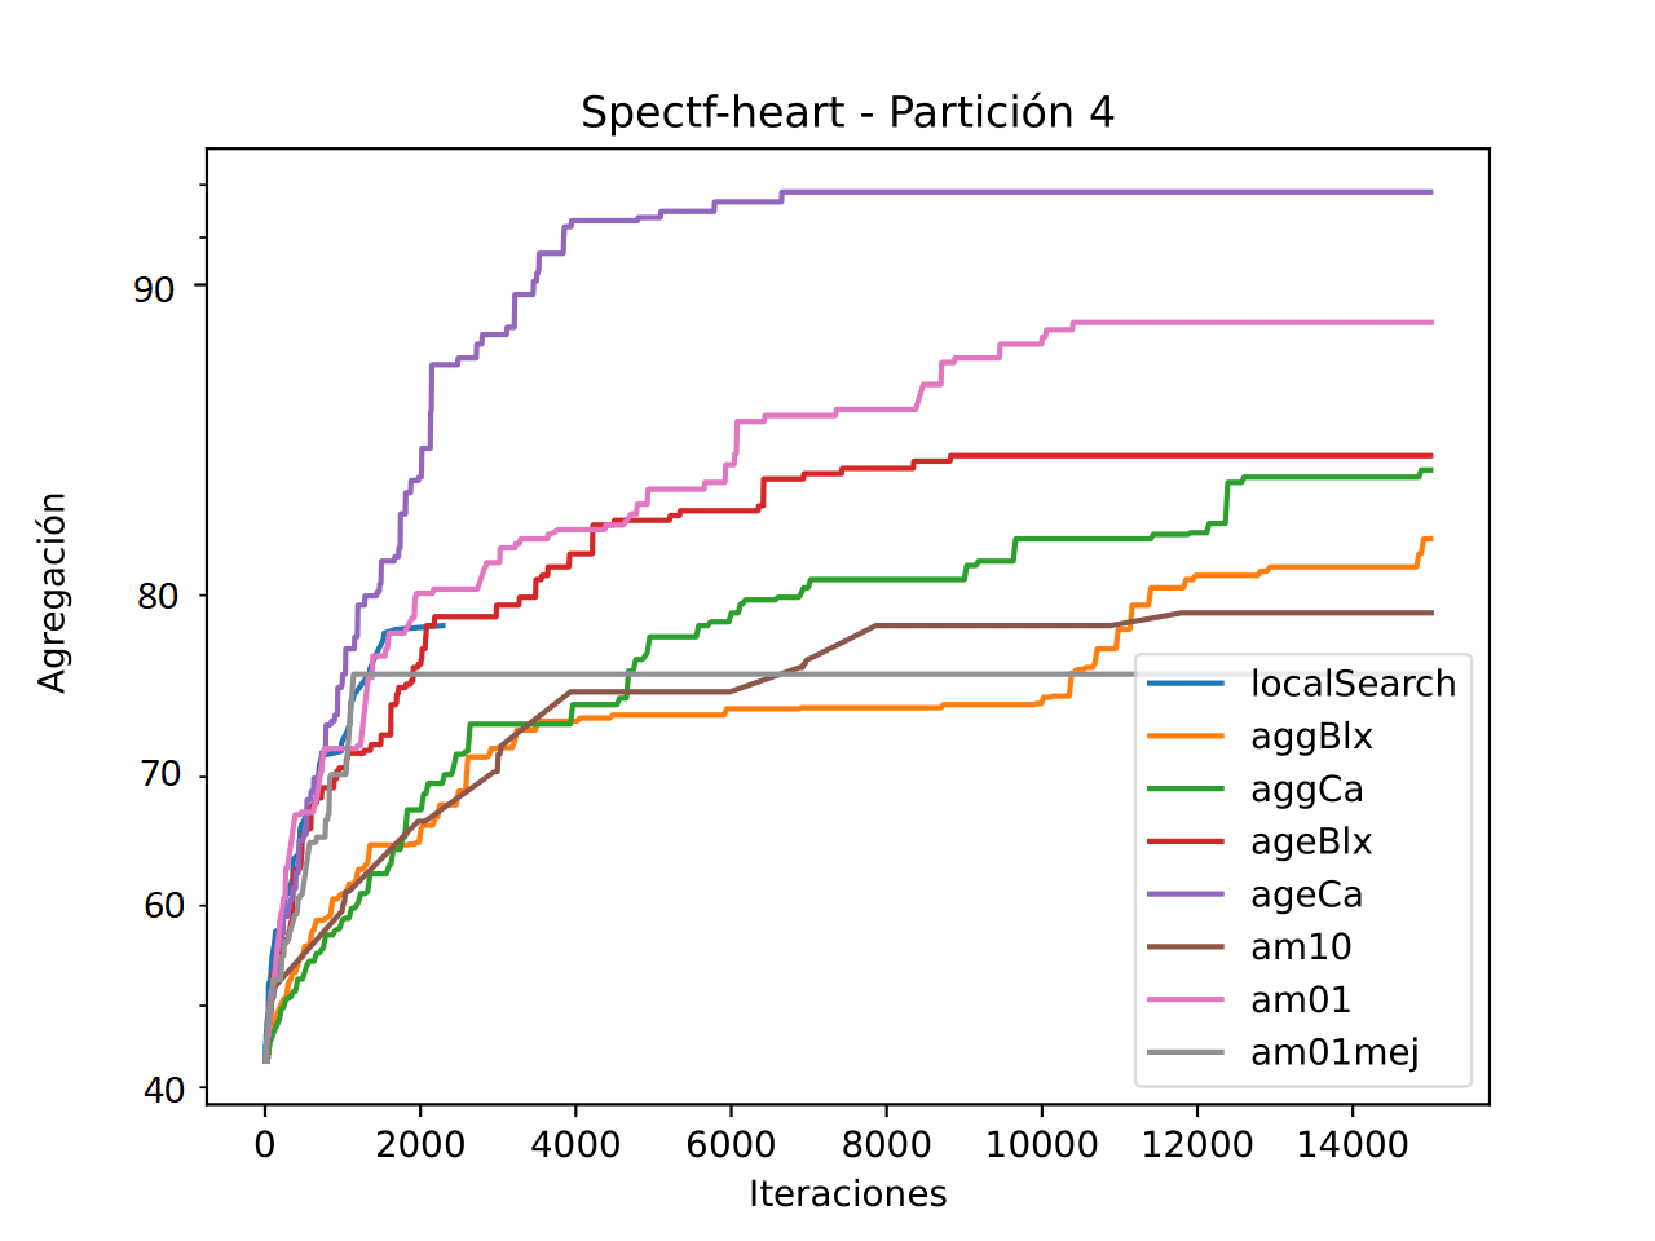
\includegraphics[width=75mm]{../FUENTES/graph/plots/spectf-heart4.pdf}}
	\subfigure{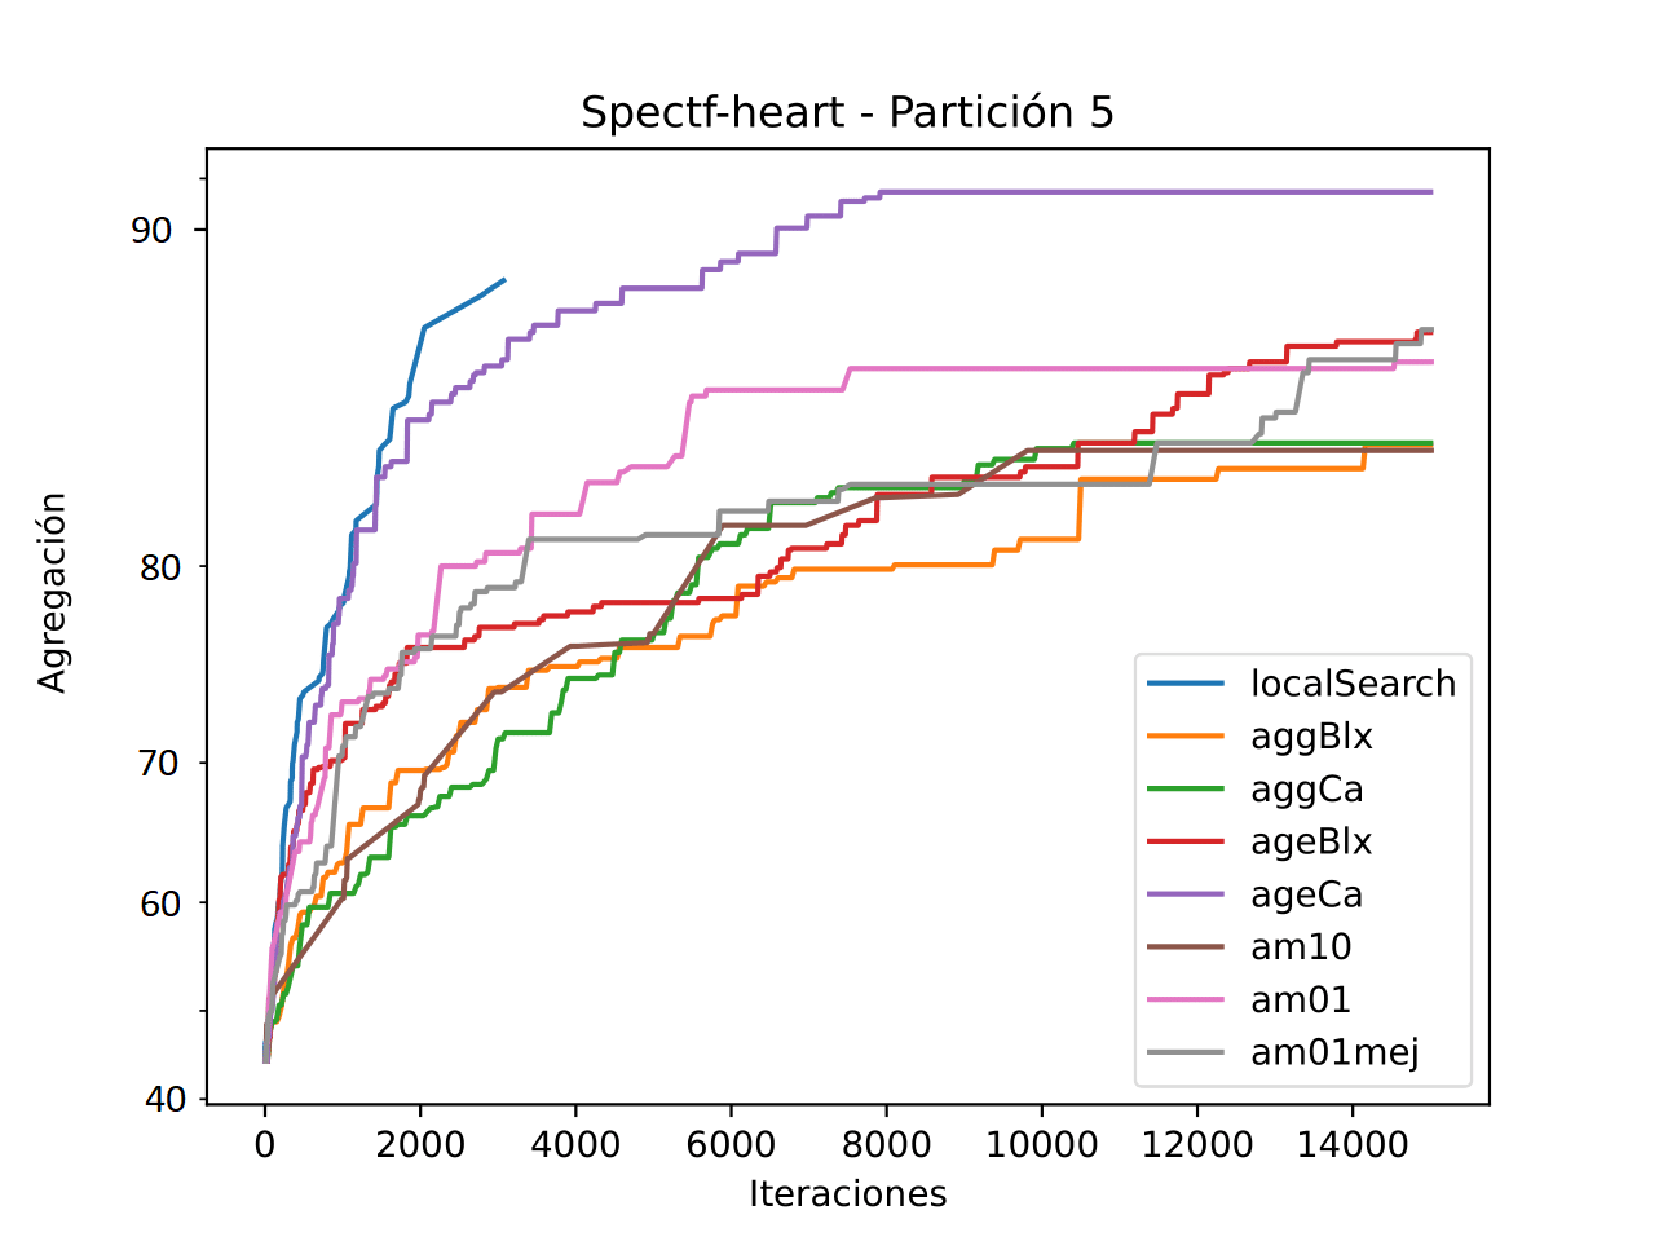
\includegraphics[width=75mm]{../FUENTES/graph/plots/spectf-heart5.pdf}}
	\caption{Gráficas de la agregación respecto al número de iteraciones con los datos de train de Spectf-heart}
\end{figure}

Hay que tener en cuenta que estas gráficas son con los datos de \emph{train}, mientras que en los resultados de las tablas previas la clasificación es de los datos de \emph{test}, por lo que aunque en alguna gráfica un algoritmo pueda parecer mejor, no tiene por qué serlo.

En todas las gráficas podemos observar a qué se debe que el algoritmo \emph{localSearch} tenga un tiempo mucho inferior: se detiene mucho antes que los demás.

En todos los algoritmos, la agregación sólo aumenta. Esto se debe a que representamos sólo la agregación de la mejor solución, y en todos los algoritmos, si en una nueva generación se genera una solución peor, no reemplaza a ninguna otra, por lo que la agregación siempre aumenta con el número de iteraciones.

Todos los algoritmos tienen comportamientos similares, aumentando mucho la agregación en las primeras iteraciones (ya que como parten de soluciones aleatorias, es fácil realizar mejores), y mejorando cada vez menos (ya que es más difícil mejorar la solución). Además, todas empiezan con una agregación entre el $40\%$ y el $50\%$. Eso se debe a que, aunque sean soluciones aleatorias, siguen siendo una modificación del algoritmo del vecino más cercano, por lo que obtenemos resultados decentes aunque sea una mala modificación.

\subsection{Análisis de los resultados}

Todos los algoritmos genéticos y meméticos dan mejores resultados que el algoritmo \emph{1-NN} y \emph{RELIEF}, principalmente debido al aumento de la tasa de reducción, aunque es a costa de un aumento en el tiempo de ejecución.

De entre los algoritmos genéticos, los generacionales suelen proporcionan mejores resultados, principalmente aumentando la tasa de reducción, sin producir un aumento en el tiempo de ejecución. Aunque el intervalo de exploración del cruce aritmético está contenido dentro del intervalo del cruce Blx, el cruce aritmético suele dar mejores resultados ya que hay infinitas posibles soluciones, y por lo cual no las exploramos todas. Además, es más probable que una solución mejor entre dos previas ya que, por algo las considerábamos como posibles soluciones, que más alejado de ellas, por eso suele producir mejores resultados el cruce aritmético. Debido a esto, el mémetico utilizará el algoritmo genético generacional con cruce aritmético como base, el cuál mejoramos añadiendo la búsqueda local.

El algoritmo memético es el que llega a producir las mejores soluciones, aunque depende de a que conjunto de soluciones le apliquemos la búsqueda local. Otra cosa a tener en cuenta es que sólo utilizamos 10 cromosomas en el algoritmo genético frente a las 30 del generacional, lo cuál nos permite una mayor exploración de cada uno (ya que le corresponden más iteraciones), pero tenemos menos cromosomas iniciales.

Además podemos ver que es mejor aplicar la búsqueda local en el algoritmo memético a soluciones aleatorias que a las mejores. Esto se debe a que estas soluciones mejores estarán cerca de un mínimo local, por lo que la búsqueda local se queda ``atascada'' y no nos proporciona mejoras, mientras que aplicarle la búsqueda local a soluciones peores permite que realicemos una mayor exploración ``saliendo'' de estos mínimos locales.

La mayoría de resultados del algoritmo memético con un $10\%$ aleatorio de la población son mejores que las del genético con cruce aritmético, en el cuál está basado. Esto nos permite ver la importancia de la búsqueda local para encontrar mejores soluciones.

Por último, comparando con la búsqueda local, podemos ver que todos los algoritmos genéticos y meméticos suponen un aumento considerable en el tiempo de ejecución. Esto se debe principalmente a que en estos algoritmos siempre realizamos las 15000 ejecuciones, mientras que en la búsqueda local terminábamos mucho antes al quedarnos atascados en un mínimo local. En caso de que eliminásemos la condición de salir si la solución no mejora en la búsqueda local, los tiempos son similares, por lo que la mayor parte del tiempo de ejecución se debe al calculo de la agregación de la solución. Pero a cambio, los resultados son mejores, por lo que si damos mayor prioridad a la calidad de la solución que al tiempo de ejecución, todos los algoritmos estudiados en esta práctica suponen una mejora.

\end{document}